\section{Base Te\'orica}\label{sec:base}

A base teórica é fundamental para se obter resultados satisfatórios, pois ela proporciona um sólido conhecimento sobre o tema em questão. Neste capítulo, são abordados diversos aspectos relevantes, incluindo métricas de erro e modelos regressivos de previsão. Essas métricas desempenham um papel crucial na avaliação e comparação dos modelos, permitindo uma análise precisa do desempenho de cada um. Além disso, os modelos regressivos de previsão são explorados, fornecendo insights valiosos sobre como essas técnicas podem ser aplicadas para realizar previsões com precisão. Compreender e dominar esses conceitos é essencial para se obter resultados confiáveis e embasar as próximas etapas do trabalho de pesquisa.



\subsection{Modelos de S\'eries Temporais Univariados}\label{subsec:arima}

A previsão de séries temporais é um desafio complexo, sem uma resposta fácil. Existem inúmeros modelos estatísticos que afirmam superar uns aos outros, mas nunca está claro qual modelo é o melhor.

Dito isto, os modelos baseados em ARMA são frequentemente uma boa opção para iniciar. Eles podem alcançar pontuações decentes na maioria dos problemas de séries temporais e são adequados como modelos de referência em tais problemas.

Quanto ao modelo ARIMA, ele é dividido em três componentes: AR (Auto-Regressão), I (Integração) e MA (Média Móvel). O componente AR leva em consideração os valores anteriores da série temporal, o componente I trata das diferenças entre os valores observados para tornar a série estacionária, e o componente MA considera os erros residuais do modelo. Esses componentes combinados ajudam a capturar os padrões e tendências presentes na série temporal.

\subsubsection{Componente Autorregressivo}

O componente autoregressivo do modelo ARIMA é representado por AR(p), em que o parâmetro p determina o número de séries temporais defasadas utilizadas.

A equação do modelo AR(p) é expressa da seguinte forma:

\begin{eqnarray}
	Y_t&=&c+\sum_{n=1}^{p} \alpha_n Y_{t-n} + \varepsilon_t\label{AR}
\end{eqnarray}

A partir dos dados, é possível obter uma previsão utilizando o modelo AR(7).

\begin{figure}[!htb]
	\centering
	\caption{Comparação dos modelos AR e ARX}
	\begin{subfigure}{1\textwidth}
		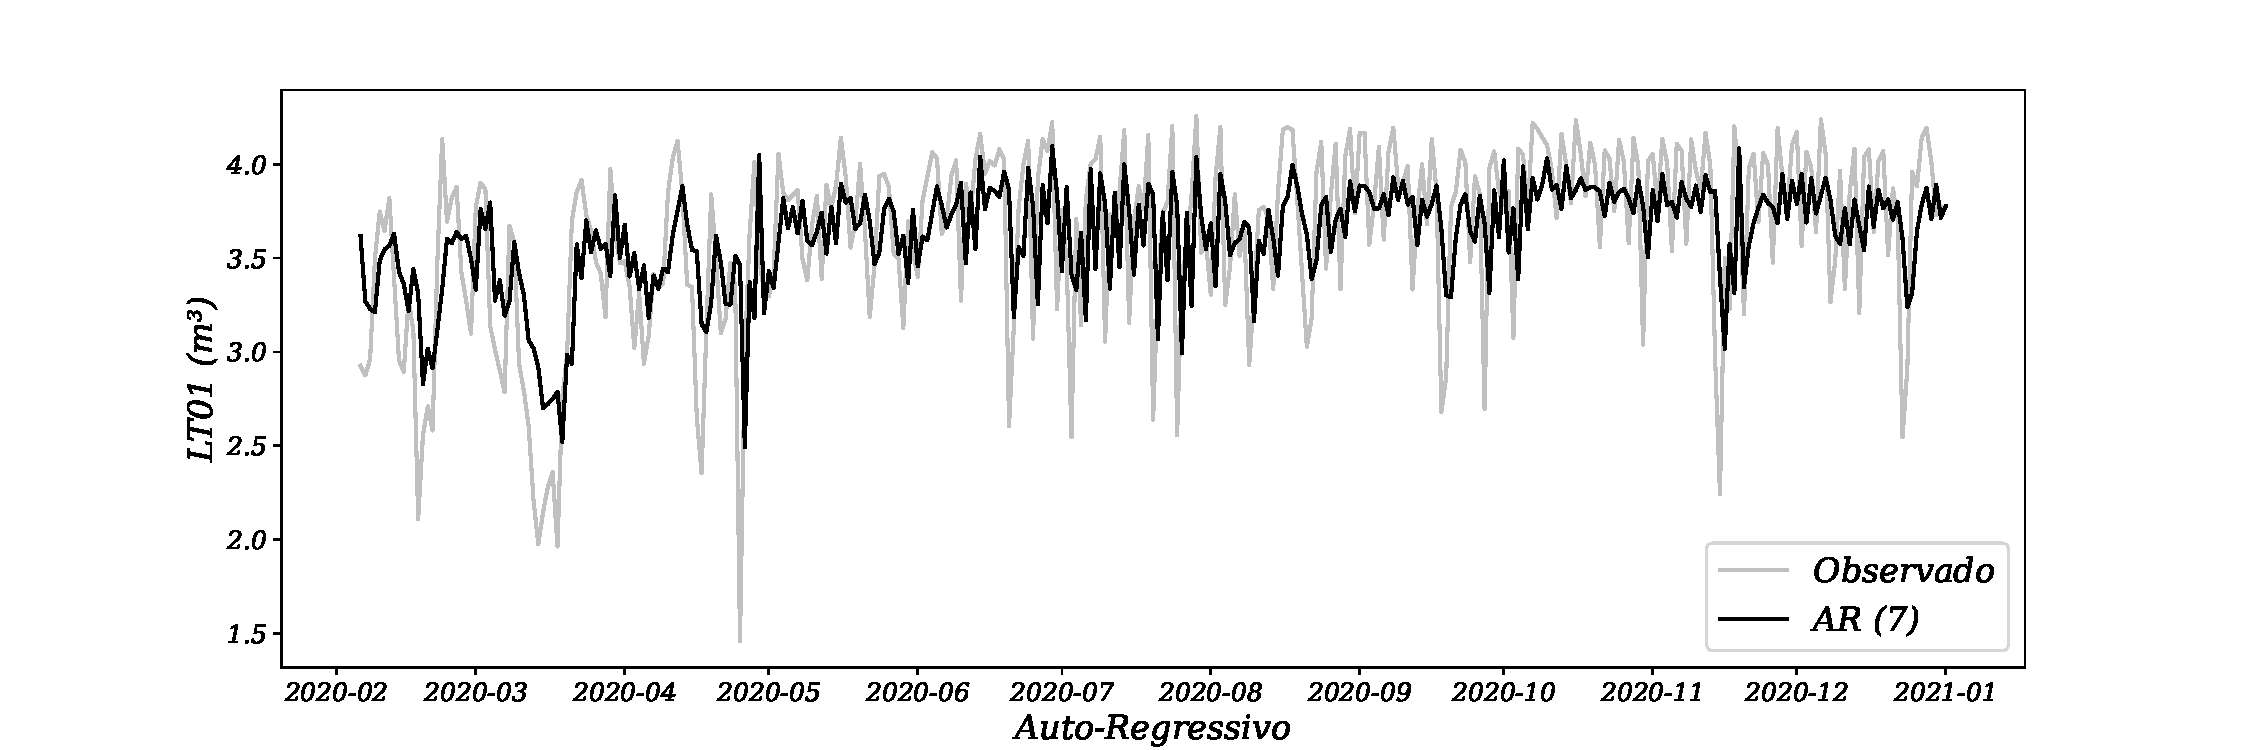
\includegraphics[width=\linewidth]{Modelos/Figuras/AR}
		\caption{Modelo AR(7)}
		\label{fig:1-ar}	
	\end{subfigure}
	
	\begin{subfigure}{1\textwidth}
		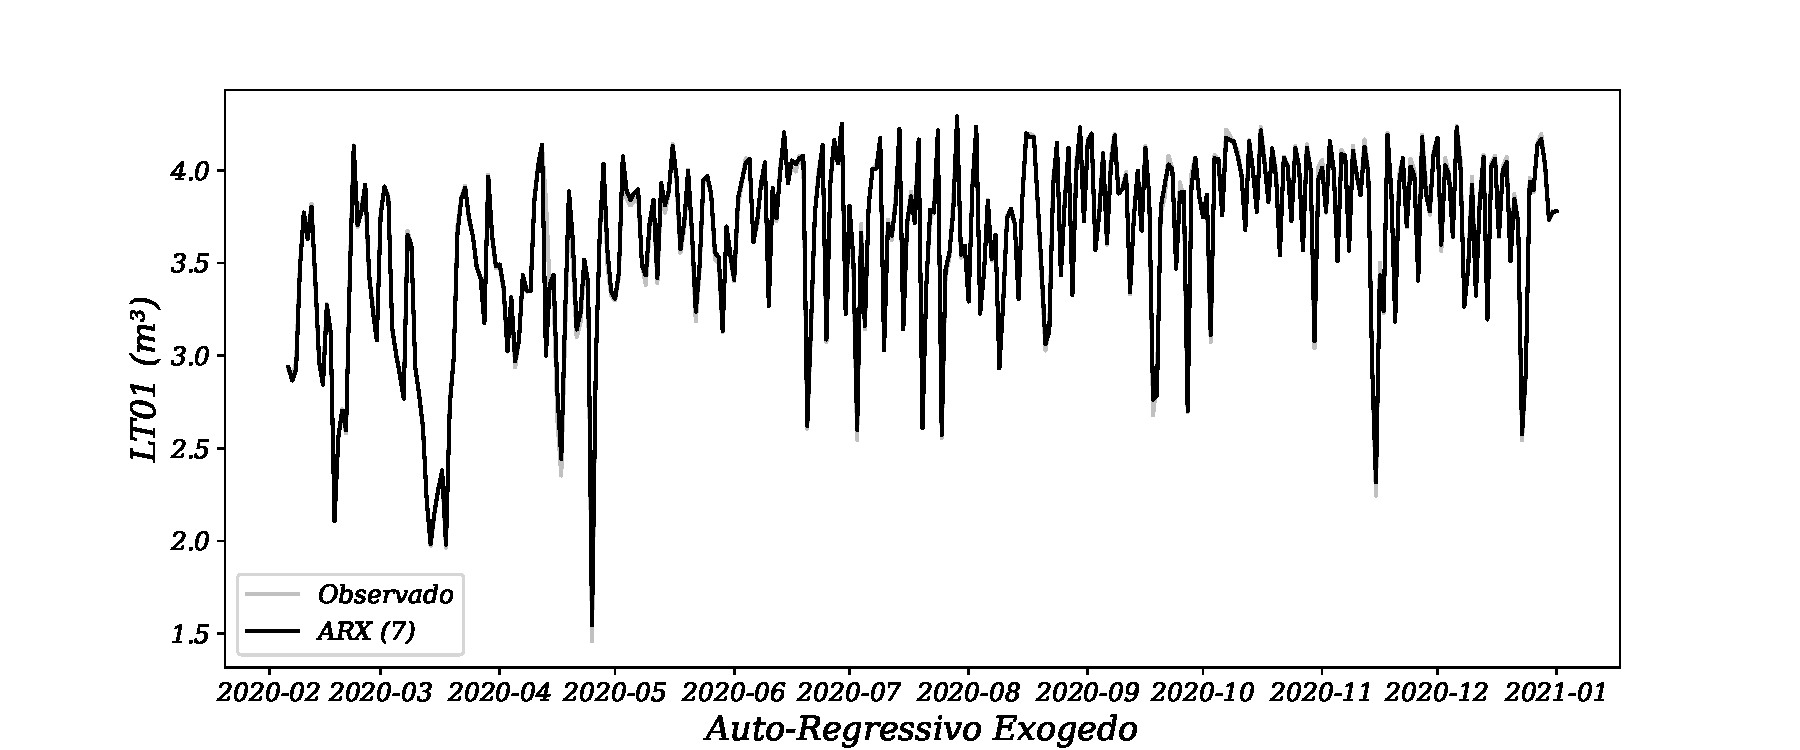
\includegraphics[width=\linewidth]{Modelos/Figuras/ARX}
		\caption{ARX (7)}
		\label{fig:1-arx}	
	\end{subfigure}
	
	\fonte{Elaboração própria a partir de dados da SANEPAR (2018 a 2020)}
\end{figure}



Na equação \eqref{AR}, o termo $\varepsilon_t$ representa o ruído branco. Essa equação pode ser entendida como uma regressão múltipla, em que os valores defasados de $y_t$ são utilizados como preditores. Esse modelo é conhecido como modelo autorregressivo de ordem $p$, ou AR(p).

A Figura \ref{fig:1-ar} tem como objetivo apresentar uma previsão de um passo à frente (um dia). Nos apêndices \ref{sec:ararxma24}, pode-se observar uma comparação entre os modelos AR, MA e ARX.

O modelo ARX é uma extensão do modelo AR, que incorpora variáveis exógenas nos dados para melhorar as previsões futuras. Esse modelo também é multivariado, como mostrado na subseção \ref{subsec:mult}, e foi incluído aqui para fins de comparação com o modelo AR simples, considerando a presença de variáveis exógenas.

Embora o modelo AR possa ser visualmente adequado para a previsão que está sendo feita, é importante destacar que, por ser um modelo autorregressivo, ele realiza previsões lineares e não captura padrões não lineares presentes nos dados. Para uma análise mais abrangente da série temporal, é necessário considerar exemplos de casos gerais.

\subsubsection{AR(0): Ru\'ido branco}

Se o parâmetro $p$ for definido como zero (AR($0$)), significa que não há termos autorregressivos no modelo. Nesse caso, a série temporal se comporta como um ruído branco. Cada ponto de dados é amostrado de uma distribuição com média zero e variância igual a sigma-quadrado. Isso resulta em uma sequência de números aleatórios que não exibem nenhum padrão ou correlação.

Essa propriedade do ruído branco pode ser útil em análises estatísticas, pois serve como uma hipótese nula. Ao comparar diferentes modelos ou testar a presença de padrões em uma série temporal, podemos usar o ruído branco como referência para avaliar se os resultados observados são estatisticamente significativos ou apenas resultado do acaso. Isso nos ajuda a evitar a detecção de padrões falsos positivos e garante a confiabilidade das análises realizadas.

\subsubsection{AR(1): Caminhadas aleat\'orias e Oscila\c c\~oes}

Com o parâmetro $p$ definido como $1$, o modelo AR leva em consideração o valor anterior da série temporal multiplicado por um coeficiente e, em seguida, adiciona ruído branco. Quando o coeficiente é igual a $0$, temos apenas ruído branco, resultando em uma série de tempo completamente aleatória, sem padrões previsíveis.

Quando o coeficiente é igual a $1$, temos uma caminhada aleatória, onde cada valor da série é obtido somando-se o valor anterior a um termo de ruído branco. Nesse caso, os valores da série apresentam uma tendência linear, aumentando ou diminuindo ao longo do tempo sem retornar à média.

Se o coeficiente estiver na faixa $0 < \alpha < 1$, temos o fenômeno de reversão média. Isso significa que os valores da série tendem a oscilar em torno de uma média central e a regressar em direção a ela após se afastarem. Esse padrão indica uma tendência de retorno à média ao longo do tempo.

Os diferentes comportamentos da série temporal, determinados pelo coeficiente no modelo AR, têm implicações importantes na análise e previsão de dados. A compreensão desses padrões é fundamental para escolher o modelo adequado e interpretar corretamente os resultados obtidos.

\subsubsection{AR(p): Termos de ordem superior}

Aumentar ainda mais o parâmetro $p$ no modelo AR significa considerar um número crescente de medições de tempo anteriores, cada uma multiplicada pelo seu próprio coeficiente. Isso permite levar em conta uma memória mais longa da série temporal e capturar padrões de dependência mais complexos ao longo do tempo.

No entanto, é importante ter em mente que aumentar excessivamente o valor de $p$ pode levar a problemas de \textit{overfitting}, onde o modelo se ajusta muito bem aos dados de treinamento, mas tem um desempenho ruim na previsão de novos dados. Portanto, é necessário encontrar um equilíbrio entre a complexidade do modelo e sua capacidade de generalização.

Além disso, é comum combinar o modelo AR com o modelo de média móvel (MA) para formar o modelo ARMA. O modelo MA considera os erros passados, ou seja, as diferenças entre os valores reais e as previsões anteriores, ajustadas por coeficientes. A combinação dos componentes AR e MA permite capturar tanto a dependência autorregressiva quanto a dependência na média móvel, proporcionando uma modelagem mais abrangente da série temporal.

Em suma, aumentar o parâmetro $p$ no modelo AR pode melhorar a capacidade do modelo de capturar padrões complexos da série temporal, mas é necessário ter cuidado para evitar \textit{overfitting}. A combinação com o modelo MA pode fornecer uma modelagem mais completa dos dados. A escolha adequada dos parâmetros depende da análise cuidadosa dos padrões presentes na série temporal e do equilíbrio entre a complexidade do modelo e sua capacidade de generalização.

\subsubsection{M\'edia M\'ovel}\label{subsubsec:ma}
No modelo de média móvel (MA), o componente não é uma média móvel simples, mas sim uma combinação de termos de erro de previsão defasados. O parâmetro $q$ no modelo MA representa o número de termos de erro de previsão que são levados em consideração na previsão.

De acordo com \citeonline{signal} este componente não é uma média de rolamento, mas sim os atrasos no ruído branco.

Em um modelo MA(1), por exemplo, a previsão é composta por um termo constante, o produto do termo de erro de previsão anterior por um multiplicador, e o termo de erro de previsão atual. Essa abordagem baseia-se em princípios estatísticos e de probabilidade, ajustando a previsão com base em termos anteriores de erro de previsão.

O modelo MA é uma alternativa ao modelo AR e é usado para capturar padrões de dependência na média móvel, ou seja, a influência de erros passados na previsão atual. Ao combinar o modelo AR e o modelo MA, como no modelo ARMA, é possível obter uma modelagem mais abrangente que considera tanto a dependência autorregressiva quanto a dependência na média móvel.

Portanto, o modelo MA leva em conta os termos de erro de previsão defasados para ajustar a previsão atual, permitindo considerar a probabilidade e estatística na modelagem da série temporal.


\begin{eqnarray}
	y_t=c+\varepsilon_t+\theta_1 \varepsilon_{t-1}+\theta_2 \varepsilon_{t-2}+\cdots+\theta_q \varepsilon_{t-q}\label{eq:ma}
\end{eqnarray}

Na equação \eqref{eq:ma}, em que $\varepsilon_t$ representa o ruído branco, esse modelo é conhecido como um modelo de média móvel $MA(q)$, em que $q$ é a ordem da média móvel. É importante ressaltar que não observamos diretamente os valores de $\varepsilon_t$, portanto, essa modelagem não se trata de uma regressão no sentido convencional.

Diferentemente de uma regressão comum em que temos variáveis explicativas observadas, no modelo $MA(q)$, estamos usando os termos de ruído branco defasados para estimar e prever os valores da série temporal. O objetivo é capturar a dependência dos termos de erro passados na previsão atual.

Esse modelo é útil para modelar séries temporais em que a média móvel tem um impacto significativo nas observações. Ao ajustar a série temporal com base nos termos de ruído branco defasados, podemos obter uma estimativa mais precisa dos valores futuros.

Embora o modelo $MA(q)$ seja diferente de uma regressão tradicional, ele é uma ferramenta estatística poderosa para modelar e prever séries temporais, levando em consideração a dependência entre os termos de erro passados.

\begin{figure}[!htb]
	\centering
	\caption{Modelo MA(7) }
	\label{fig:1-ma}
	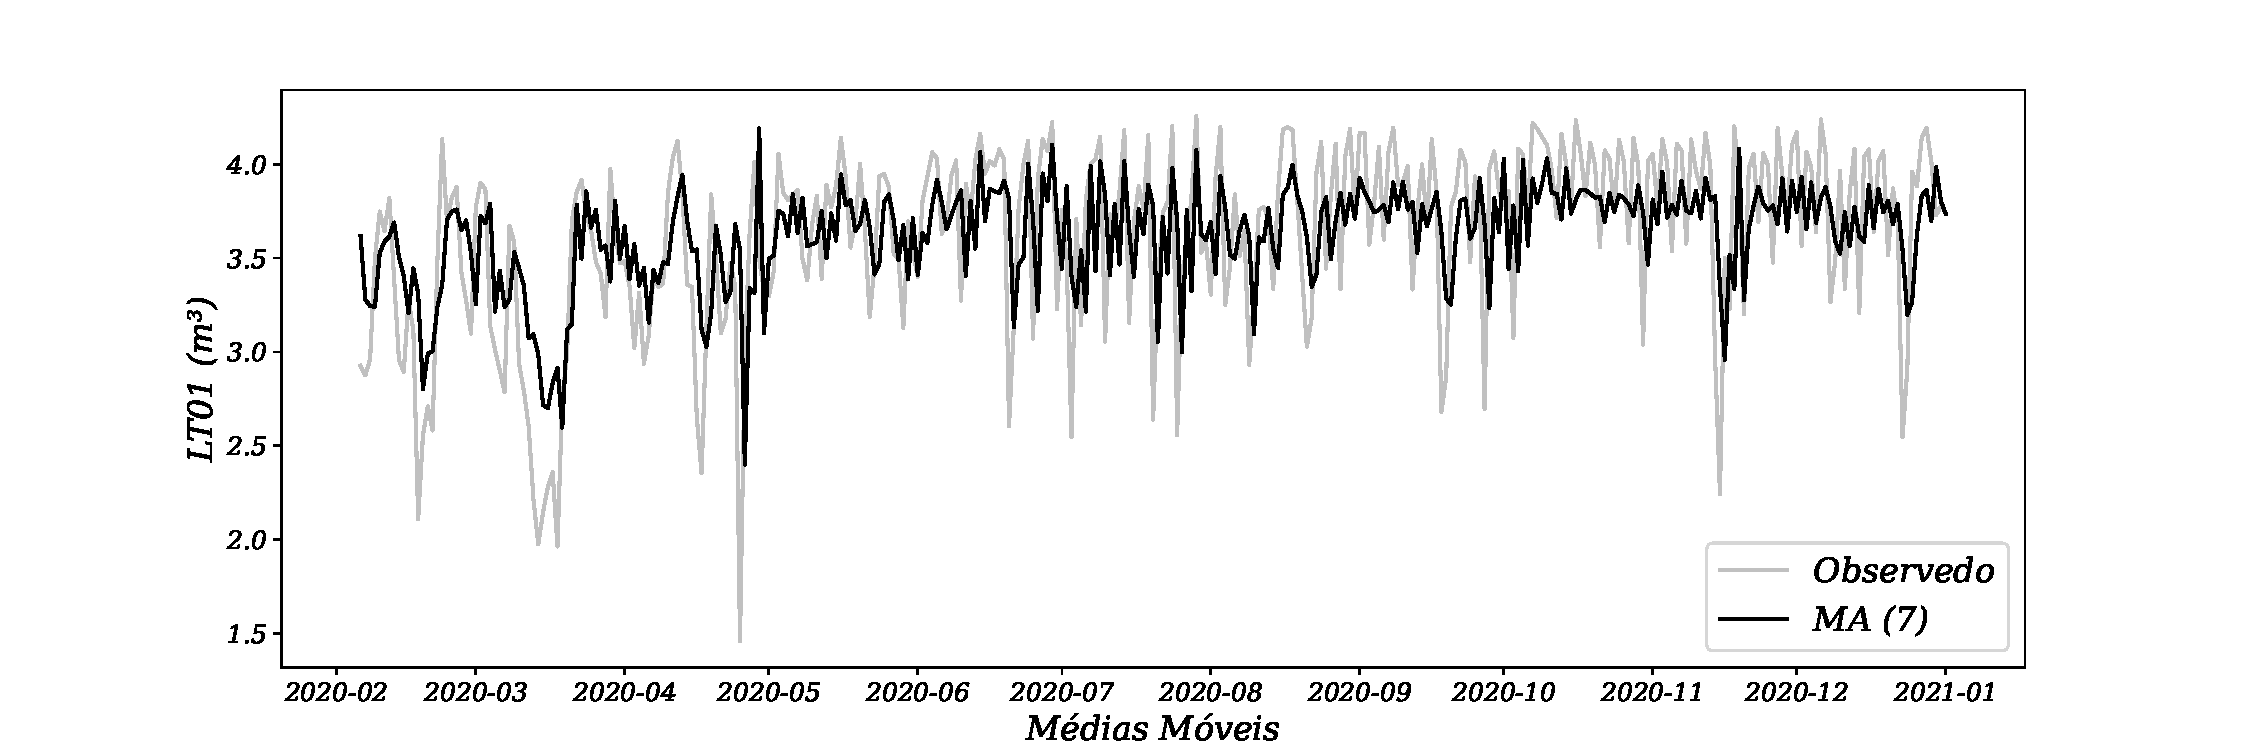
\includegraphics[width=1\linewidth]{Modelos/Figuras/MA}
	
	\fonte{Elaboração própria a partir de dados da SANEPAR (2018 a 2020)}
\end{figure}

O modelo MA, quando comparado com o modelo AR de mesma ordem, facilita a previsão. Conforme ilustrado na Figura \ref{fig:1-ma}, a previsão gráfica se assemelha ao modelo apresentado na Figura \ref{fig:1-ar}, embora não seja comparável ao modelo exibido na Figura \ref{fig:1-arx}. É importante notar que esse modelo aparenta prever com precisão o período de tempo que foi considerado.

\subsubsection{Modelos ARMA e ARIMA}\label{subsubsec:arma}
A arquitetura ARMA é uma combinação dos modelos AR  e MA, onde o modelo AR é adicionado ao modelo MA.

No modelo ARMA, é adicionada uma constante à soma dos termos autorregressivos multiplicados pelos seus coeficientes, juntamente com a soma dos termos de média móvel multiplicados pelos seus coeficientes, além do ruído branco. Essa estrutura é amplamente utilizada em diversos modelos de previsão em diferentes áreas.

\begin{figure}[!htb]
	\centering
	\caption{ARMA (7,7)}
	\label{fig:1-arma}
	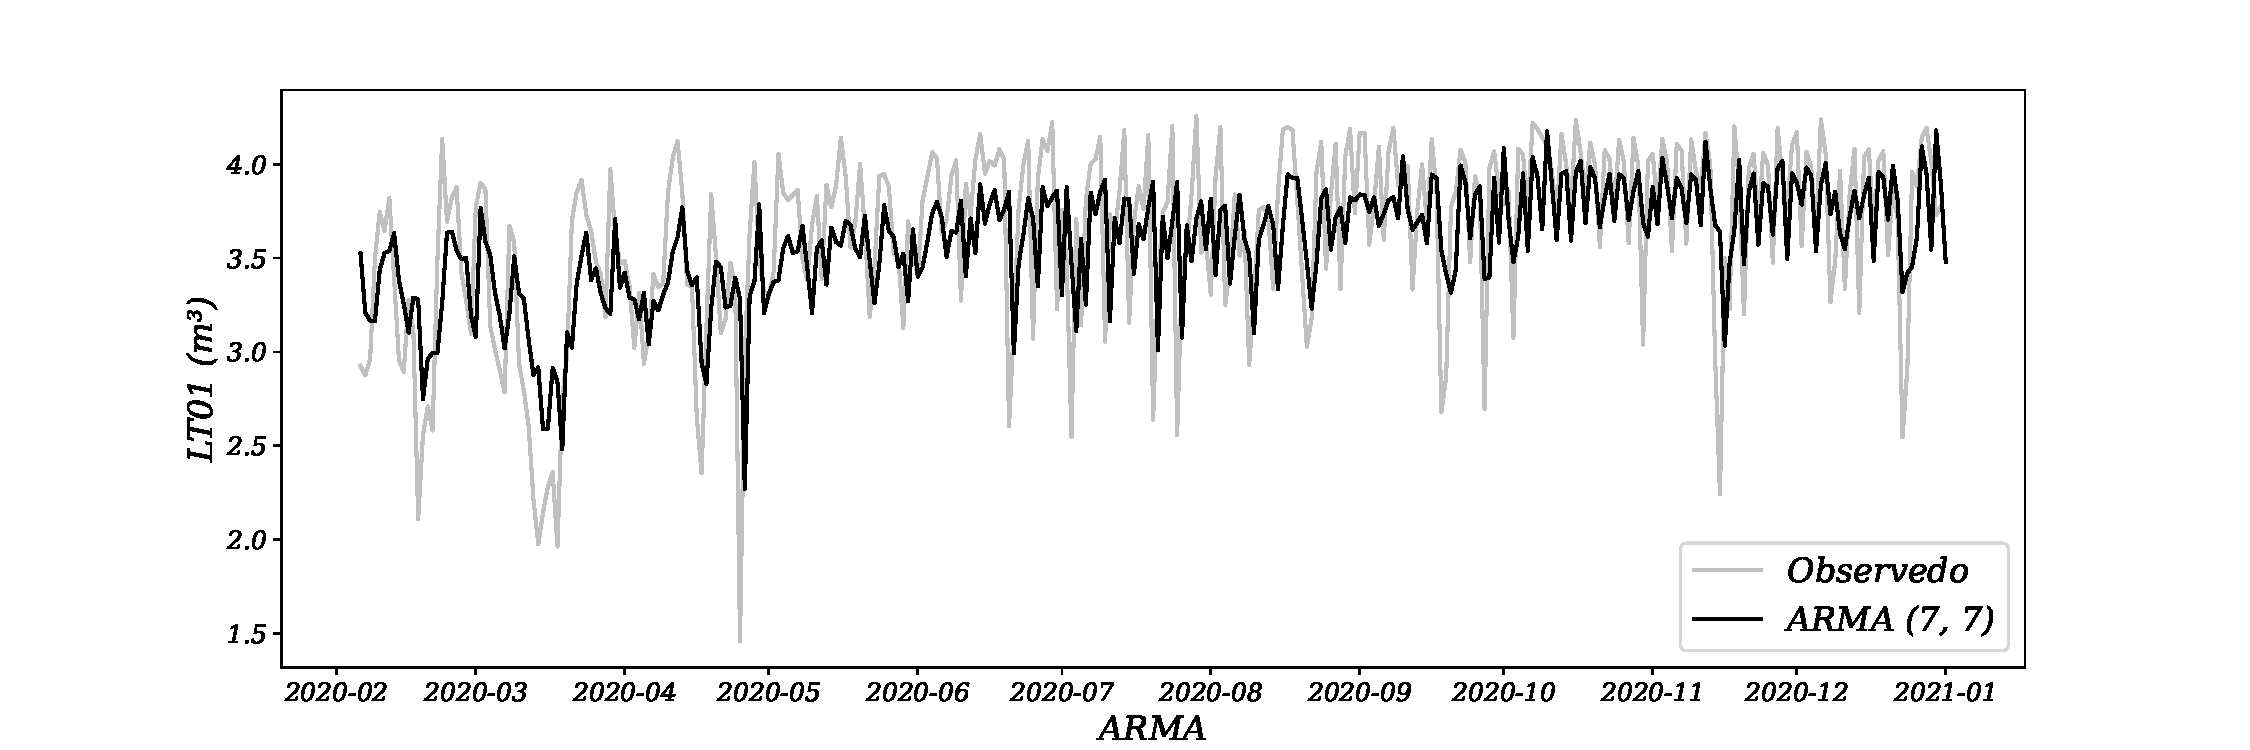
\includegraphics[width=1\linewidth]{Modelos/Figuras/ARMA}
	
	\fonte{Elaboração própria a partir de dados da SANEPAR (2018 a 2020)}
\end{figure}

A Figura \ref{fig:1-arma} ilustra a combinação dos modelos AR e MA em um modelo ARMA. Essa abordagem pode levar a uma redução significativa no erro de previsão, como observado nos apêndices \ref{sec:comtb24} e \ref{sec:comtb18}, onde são apresentadas comparações com um maior número de passos de previsão.

\subsubsection{ARIMA}

\begin{eqnarray}
	Y_t = \beta_2 + \omega_1\varepsilon_{t-1} + \omega_2 \varepsilon_{t-2} +\ldots+ \omega_q \varepsilon_{t-q} + \varepsilon_t \label{arima}
\end{eqnarray}

Na equação \eqref{arima}, a variável $Y_t$ representa a série temporal que foi diferenciada (possivelmente mais de uma vez). Os ``preditores'' no lado direito da equação incluem os valores defasados de $Y_t$ e os erros defasados. Esse tipo de modelo é conhecido como ARIMA ($p, d, q$).

O modelo ARIMA é uma extensão do modelo ARMA que incorpora uma etapa adicional de pré-processamento chamada de diferenciação. Essa etapa é representada pela notação \textbf{I(d)}, em que \textbf{d} denota a ordem de diferenciação, ou seja, o número de transformações necessárias para tornar a série temporal estacionária. Portanto, um modelo ARIMA é simplesmente um modelo ARMA aplicado à série temporal diferenciada. Isso permite lidar com séries temporais que possuem tendências ou padrões não estacionários.

\begin{figure}[!htb]
	\centering
	\caption{ARIMA (7,1,7)}
	\label{fig:1-arima}
	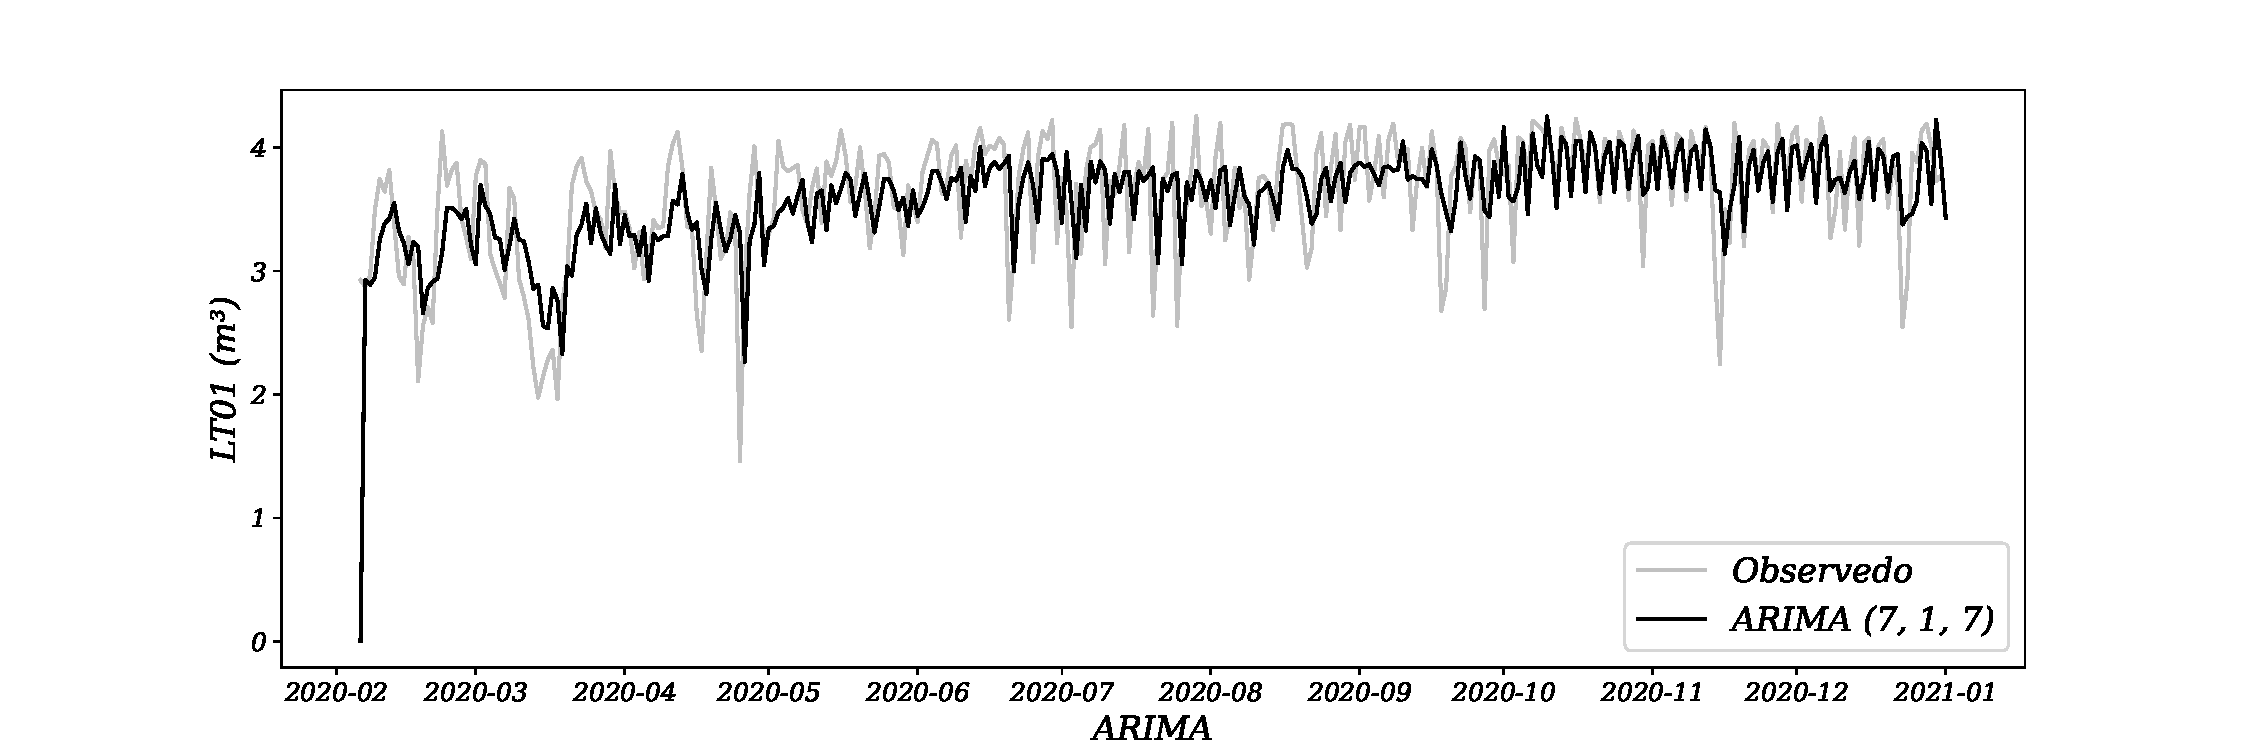
\includegraphics[width=1\linewidth]{Modelos/Figuras/ARIMA}
	
	Fonte: Elaboração própria a partir de dados da SANEPAR (2018 a 2020)
\end{figure}

Ao analisar a Figura \ref{fig:1-arima}, não se nota uma diferença visual significativa em relação aos outros métodos apresentados anteriormente. O método ARX ainda parece ser superior aos demais com base na análise visual.

Embora os modelos ARIMA sejam eficazes, incorporar variáveis sazonais e exógenas ao modelo pode potencializar sua capacidade de previsão. No entanto, é importante destacar que o modelo ARIMA pressupõe que a série temporal seja estacionária. Quando lidamos com séries temporais não estacionárias, é necessário recorrer a outros modelos para a análise e previsão adequadas.

\subsubsection{SARIMA}

\begin{eqnarray}
	Y_t&=&c+\sum_{n=1}^p \alpha_n y_{t-n}+\sum_{n=1}^q \theta_n \epsilon_{t-n}+\sum_{n=1}^P \phi_n y_{t-s n}+\sum_{n=1}^Q \eta_n \epsilon_{t-s n}+\epsilon_t \label{sarima}
\end{eqnarray}

O modelo proposto é uma extensão do modelo ARIMA, com a adição de componentes autorregressivos e de média móvel sazonal. Esses componentes extras são ajustados levando em consideração os padrões sazonais presentes nos dados, utilizando atrasos correspondentes à frequência sazonal (por exemplo, 12 para dados mensais). Essa abordagem permite capturar e modelar de forma mais precisa as variações sazonais e melhorar a qualidade das previsões em séries temporais com esse comportamento cíclico.

\begin{figure}[!htb]
	\centering
	\caption{SARIMA $(7,1,7) (2,1,1)_{12}$}
	\label{fig:1-sarima}
	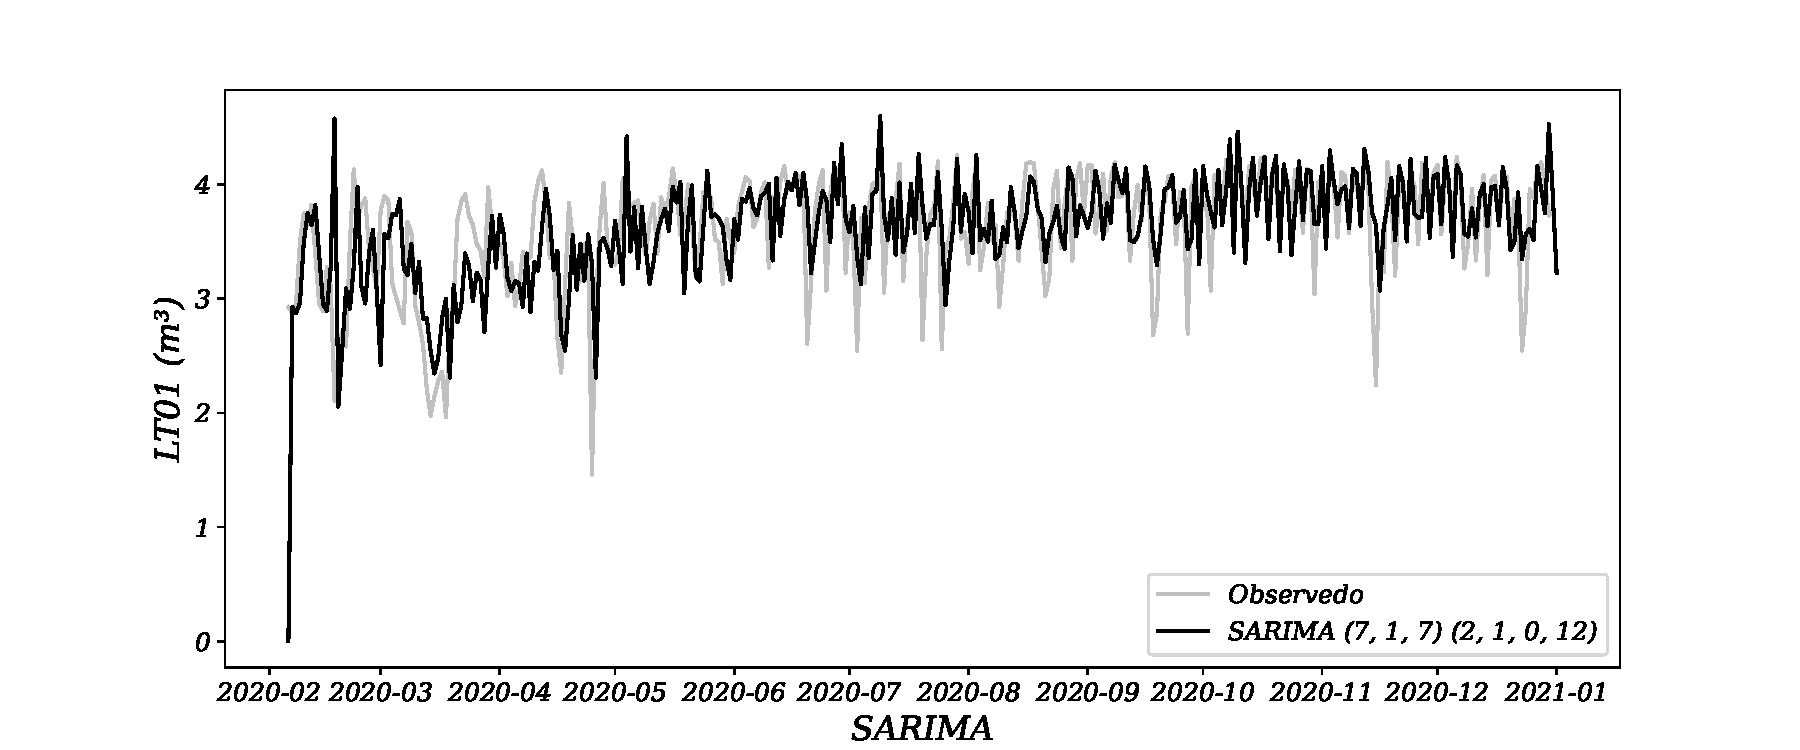
\includegraphics[width=1\linewidth]{Modelos/Figuras/SARIMA}
	
	\fonte{Elaboração própria a partir de dados da SANEPAR (2018 a 2020)}
\end{figure}

Na Figura \ref{fig:1-sarima}, é possível observar que a previsão em vermelho está mais próxima dos valores observados em preto, mostrando que a inclusão do componente de sazonalidade melhora a qualidade da previsão. Os modelos SARIMA são capazes de lidar com dados que apresentam padrões sazonais, permitindo a diferenciação dos dados em termos de componentes sazonais e não sazonais. Uma abordagem útil para determinar os melhores parâmetros do modelo é utilizar uma estrutura de pesquisa automatizada de parâmetros, como o pmdarima, que auxilia na identificação dos parâmetros ideais para o modelo SARIMA. Isso pode contribuir para uma melhor compreensão e ajuste do modelo aos dados observados.

\subsection{Modelos de S\'erie Temporal Multivariada}\label{subsec:mult}

Os Modelos de Série Temporal Multivariada são uma abordagem estatística utilizada para analisar e prever dados que possuem múltiplas variáveis dependentes ao longo do tempo. Nesse tipo de modelo, considera-se a interdependência entre as diferentes séries temporais, permitindo a análise conjunta e a identificação de padrões e relações entre as variáveis. Esses modelos são aplicados em diversas áreas, como economia, finanças, meteorologia e análise de dados, proporcionando insights valiosos para a compreensão e previsão de fenômenos complexos ao longo do tempo.

\subsubsection{ARIMAX e SARIMAX}

\begin{eqnarray}
	d_t=c+\sum_{n=1}^p \alpha_n d_{t-n}+\sum_{n=1}^q \theta_n \epsilon_{t-n}+\sum_{n=1}^r \beta_n x_{n_t}+\sum_{n=1}^P \phi_n d_{t-s n}+\sum_{n=1}^Q \eta_n \epsilon_{t-s n}+\epsilon_t \label{eq:sarmax}
\end{eqnarray}

Em \eqref{eq:sarmax}, o modelo SARIMAX é apresentado. Nesse modelo, são consideradas variáveis exógenas, ou seja, são utilizados dados externos para a realização das previsões. É importante ressaltar que mesmo que essas variáveis exógenas sejam indiretamente modeladas no histórico de previsões do modelo, ao incluí-las diretamente, o modelo será capaz de responder de forma mais ágil aos efeitos dessas variáveis. Isso significa que a incorporação de informações externas possibilita uma resposta mais rápida e precisa do modelo em relação aos fatores externos, resultando em previsões mais atualizadas e acuradas.

\begin{figure}[!htb]
	\centering
	\caption{Comparação entre ARIMAX e SARIMAX}
	\begin{subfigure}{1\textwidth}
		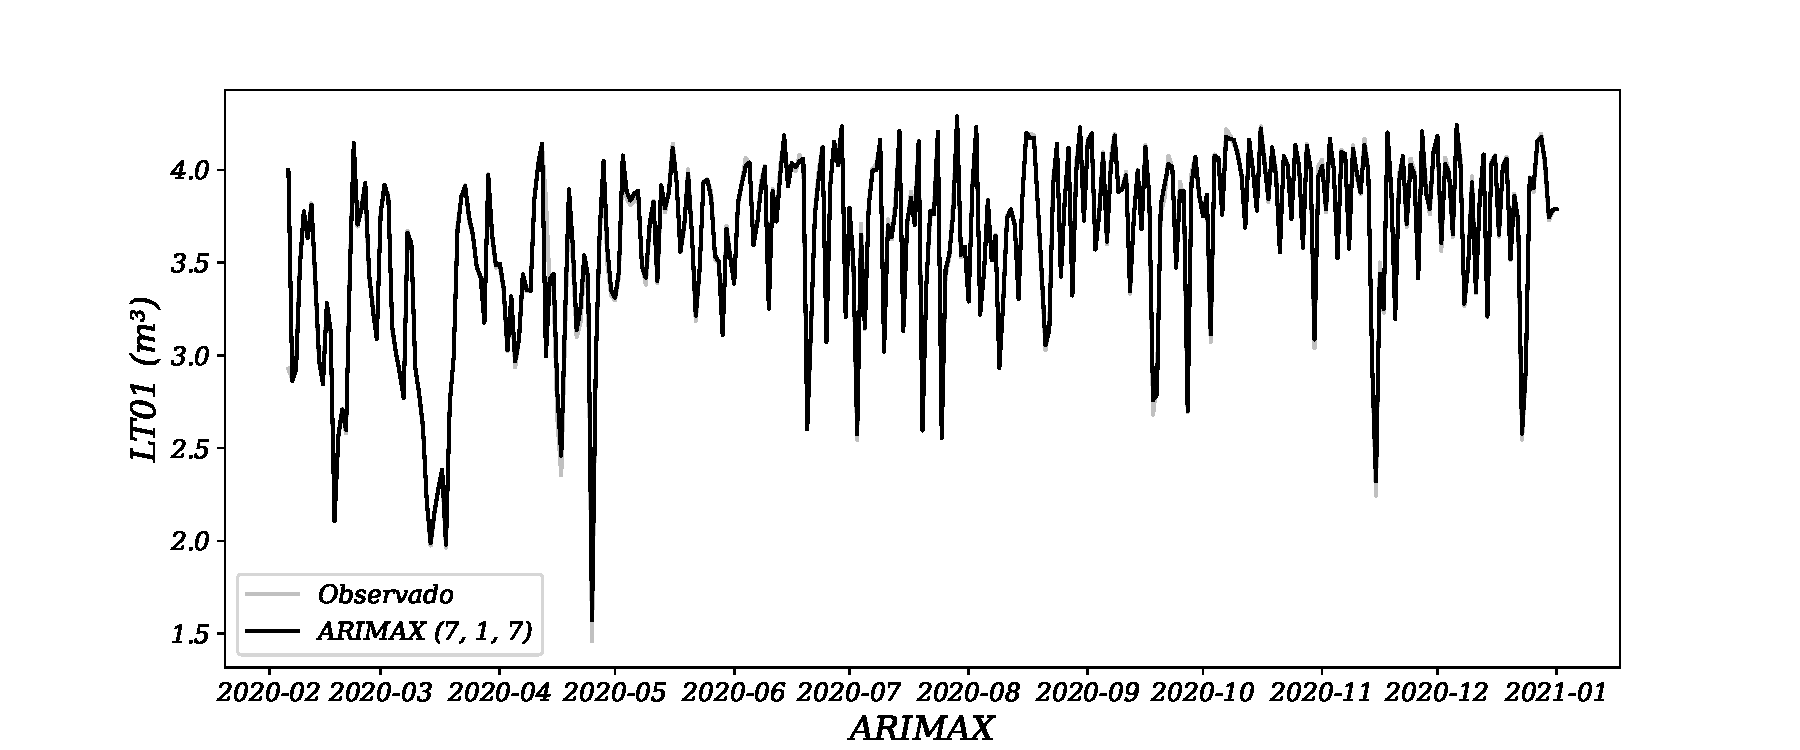
\includegraphics[width=\linewidth]{Modelos/Figuras/ARIMAX}
		\caption{ARIMAX $(7,1,7)$}
		\label{fig:1-arimax}
	\end{subfigure}
	\hfill
	
	\begin{subfigure}{1\textwidth}
		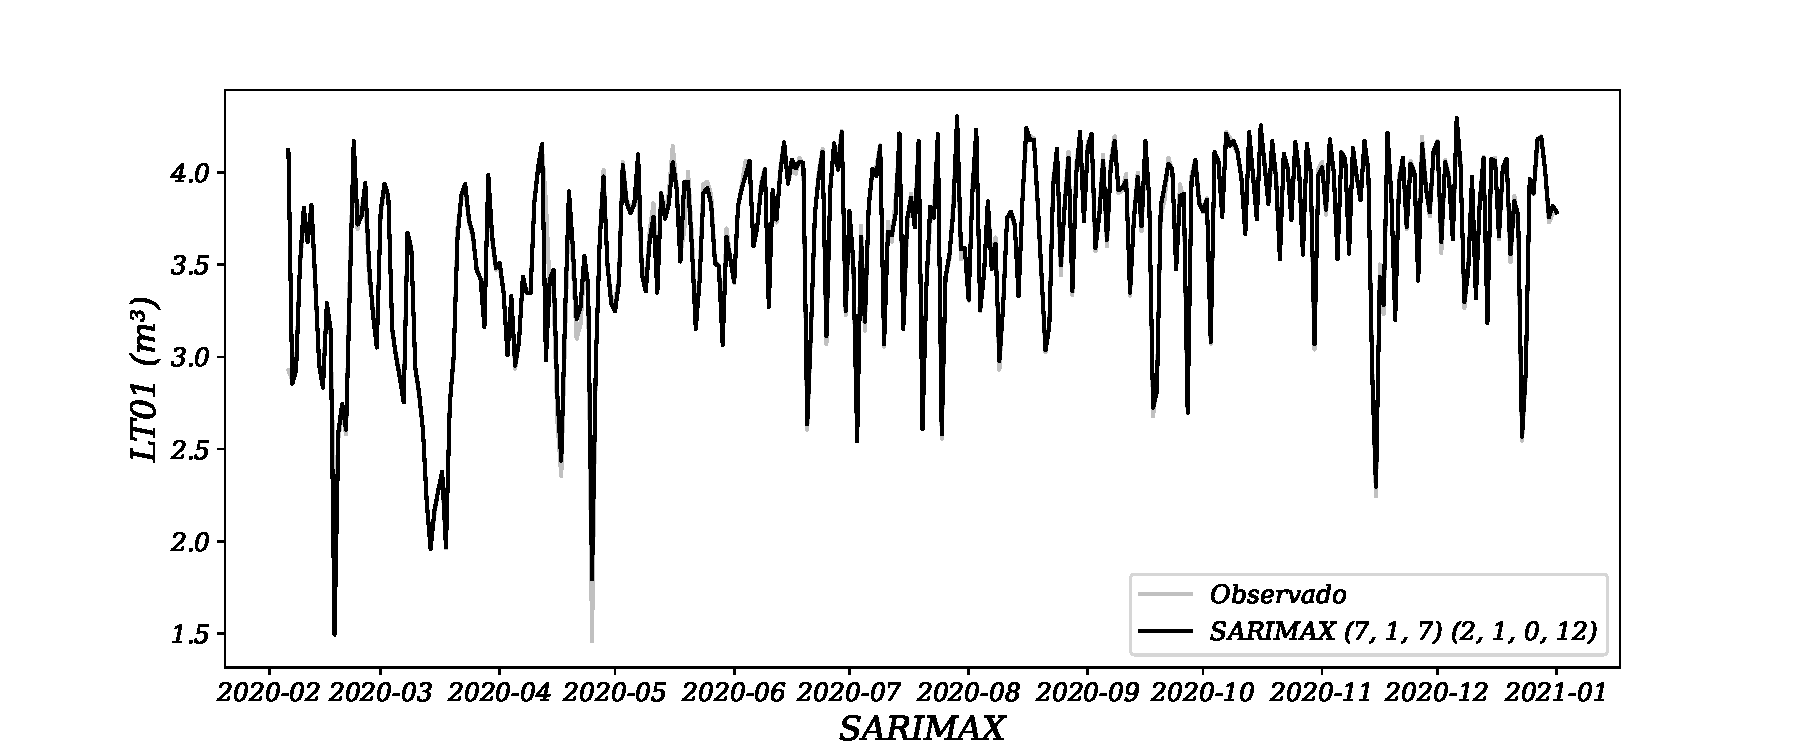
\includegraphics[width=\linewidth]{Modelos/Figuras/SARIMAX}
		\caption{SARIMAX $(7,1,7) (2,1,1)_{12}$}
		\label{fig:1-sarimax}	
	\end{subfigure}

		
	\fonte{Elaboração própria a partir de dados da SANEPAR (2018 a 2020)}
\end{figure}


Entre os modelos com variáveis exógenas, como mostrado nas Figuras \ref{fig:1-arimax} e \ref{fig:1-sarimax}, observa-se uma melhora significativa na qualidade das previsões em comparação com os modelos que não incluem variáveis exógenas. A adição dessas variáveis externas permite capturar melhor as influências e os padrões presentes nos dados, resultando em previsões mais completas e precisas. Essa inclusão de informações adicionais contribui para uma compreensão mais abrangente do comportamento da série temporal e possibilita uma melhor adaptação do modelo aos padrões observados.


\subsection{Modelos de Aprendizado de M\'aquina Supervisionados}\label{subsec:reg}

Os modelos regressivos para séries temporais têm sido amplamente reconhecidos e utilizados na literatura atual, especialmente aqueles baseados em métodos de gradiente. Esses modelos, incluindo a regressão linear simples, têm se destacado como uma escolha popular em competições de séries temporais em todo o mundo.

Esses modelos são valorizados por sua capacidade de capturar relações complexas e não lineares nos dados, permitindo previsões mais precisas e eficientes. Sua popularidade reflete o reconhecimento da eficácia desses modelos em abordar uma ampla gama de problemas de previsão de séries temporais em diferentes áreas de estudo.

A abordagem regressiva, combinada com técnicas de otimização baseadas em gradiente, tem se mostrado particularmente eficaz na obtenção de resultados de alta qualidade. Esses modelos são capazes de aprender a partir dos dados históricos e ajustar seus parâmetros de forma iterativa, otimizando assim o desempenho da previsão.

Com a crescente disponibilidade de dados e avanços na área de aprendizado de máquina, espera-se que os modelos regressivos para séries temporais continuem a evoluir e desempenhar um papel importante na análise e previsão de dados temporais em diversas aplicações.

\subsubsection{Regress\~ao Linear (LR)}

De acordo com o estudo realizado por \citeonline{korstanje2021}, nos modelos de aprendizado de máquina supervisionados, é feita uma tentativa de identificar as relações existentes entre diferentes variáveis:


\begin{itemize}
	\item Variável de destino: a variável que você tenta prever
	\item Variáveis explicativas: Variáveis que ajudam você a prever o alvo variável
\end{itemize}

Para realizar previsões, é importante que se compreenda quais tipos de variáveis explicativas podem ser utilizadas. Neste exemplo, a variável \textbf{Pressão de Sucção (PT01SU)} será considerada como a variável $x$, enquanto a variável \textbf{Nível do Reservatório (Câmara 1) LT01} será considerada como a variável $y$, com base na análise de correlação de Pearson ilustrada na Figura \ref{fig:person}. O coeficiente de correlação indica a relação entre o eixo $x$ e $y$, como expresso pela seguinte fórmula.



A fórmula do coeficiente de correlação de Pearson é dada por:

\begin{equation}
	r=\frac{\sum\left(x_i-\bar{x}\right)\left(y_i-\bar{y}\right)}{\sqrt{\left(\sum\left(x_i-\bar{x}\right)^2\right)\left(\sum\left(y_i-\bar{y}\right)^2\right)}}
\end{equation}

Onde $x_i$ e $y_i$ representam os valores das variáveis $X$ e $Y$, respectivamente. $\bar{x}$ e $\bar{y}$ são as médias dos valores $x_i$ e $y_i$. O coeficiente de correlação de Pearson mede a força e a direção da relação linear entre as variáveis $X$ e $Y$. Valores próximos a 1 indicam uma correlação positiva forte, valores próximos a -1 indicam uma correlação negativa forte, e valores próximos a 0 indicam uma ausência de correlação entre as variáveis.

\begin{figure}[H]
	\centering
	\caption{Corelação de Pearson}
	\label{fig:person}
	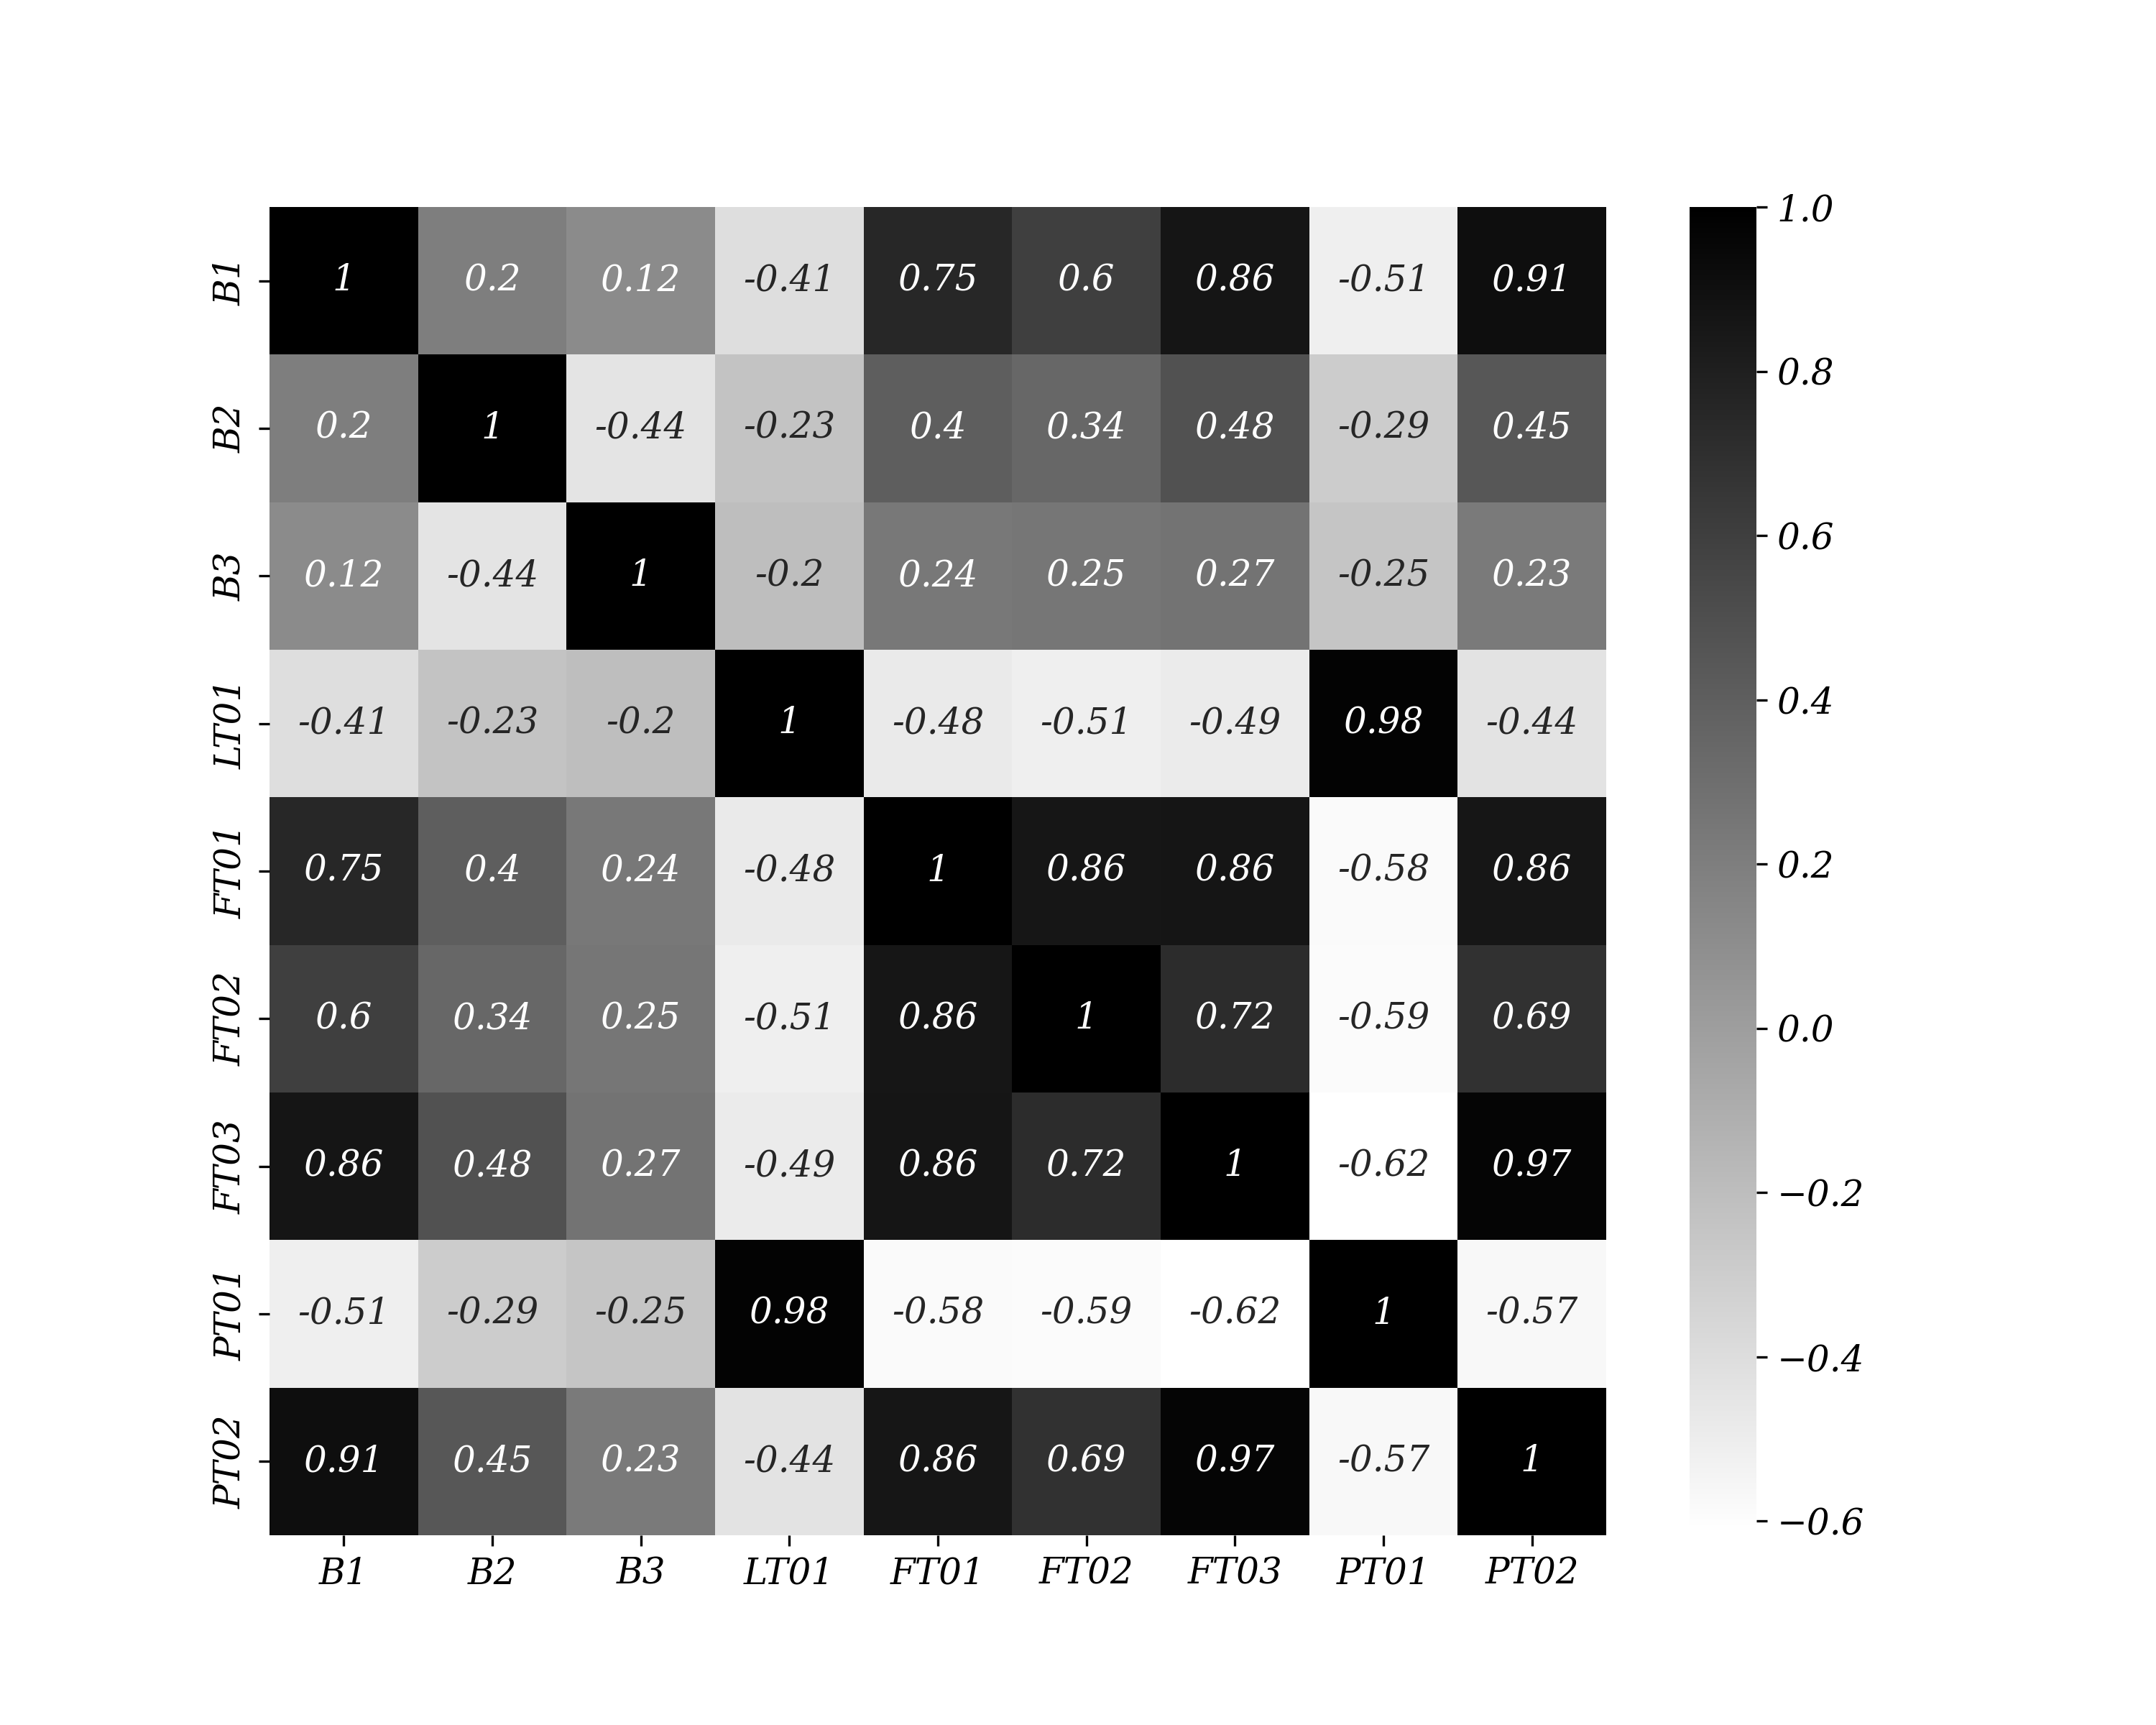
\includegraphics[width=0.9\linewidth]{Apendices/Figuras/modelagem-24h/person}
	
	Fonte: Elaboração própria a partir de dados da SANEPAR (2018 a 2020)
\end{figure}

A Figura \ref{fig:person} ilustra a correlação entre as variáveis no conjunto de dados em questão. Essa imagem representa graficamente a relação entre as variáveis e é usada para demonstrar a existência de uma correlação forte entre elas. Com base nessa análise, é possível responder à pergunta de pesquisa \ref{q1}, pois a correlação entre as variáveis é significativa.

\subsubsection{Defini\c c\~ ao do modelo}

A regressão linear é definida da seguinte forma:

\begin{equation}
	y = \beta_0 + \beta_1 x_1 + \cdots + \beta_p x_p + \varepsilon \label{eq:lr}
\end{equation}

Da Equação \eqref{eq:lr}, temos as seguintes variáveis:

\begin{itemize}
	\item Há $p$ variáveis explicativas, denotadas por $x$.
	\item Existe uma variável alvo, denotada por $y$.
	\item O valor de $y$ é calculado como uma constante $\beta_0$, somada aos valores das variáveis $x$ multiplicados por seus coeficientes $\beta_1$ a $\beta_p$.
\end{itemize}

\begin{figure}[H]
	\centering
	\caption{Regressão linear LT01 vs PT01 correlação 98\%}
	\label{fig:lr-lt01-m3}
	\includegraphics[width=0.9\linewidth]{"Modelos/Figuras/LR LT01 (m³)"}
	
	Fonte: Elaboração própria a partir de dados da SANEPAR (2018 a 2020)
\end{figure}



A Figura \ref{fig:lr-lt01-m3} fornece uma representação visual da interpretação dos coeficientes $\beta_0$ e $\beta_1$. Ela ilustra que um aumento de $1$ na variável $x$ está associado a um aumento proporcional de $\beta_1$ na variável $y$. O valor de $\beta_0$ representa o valor de $y$ quando $x$ é igual a $0$.

Para utilizar a regressão linear, é necessário estimar os coeficientes (betas) com base em um conjunto de dados de treinamento. Esses coeficientes podem ser estimados por meio da seguinte fórmula, expressa em notação matricial:

\begin{eqnarray}
	\hat{\beta}&=&\left(X^T X\right)^{-1} X^T y\label{eq:ols}
\end{eqnarray}

A fórmula mencionada, conhecida como \textbf{OLS} (método dos mínimos quadrados ordinários), é amplamente utilizada na regressão linear \citeonline{korstanje2021}. Esse método é conhecido por ser rápido de ajustar, pois requer apenas cálculos matriciais para estimar os coeficientes $\beta$. No entanto, ele é mais adequado para processos lineares e pode ser menos adequado para modelos mais complexos que envolvam relações não-lineares. Portanto, é importante considerar suas limitações ao aplicar a regressão linear em contextos mais complexos.

\begin{figure}[H]
	\centering
	\caption{Regressão linear (LR) um passo a frente}
	\label{fig:1-regressao-linear}
	\includegraphics[width=0.9\linewidth]{Modelos/Figuras/0-regressão-linear}
	
	Fonte: Elaboração própria a partir de dados da SANEPAR (2018 a 2020)
\end{figure}


\subsubsection{Floresta Aleat\'oria (Random Forest)} \label{subsubsec:rf}

Pode-se observar que ter exatamente a mesma árvore de decisão repetidas vezes não adiciona valor significativo em comparação a usar essa mesma árvore de decisão apenas uma vez. Em modelos de conjunto, cada modelo individual deve ser ligeiramente diferente dos demais. Existem dois métodos amplamente reconhecidos para criar conjuntos: o ensacamento (\textit{bagging}) e o reforço (\textit{boosting}). A floresta aleatória utiliza o ensacamento para criar um conjunto de árvores de decisão, onde cada árvore é construída com uma amostra aleatória do conjunto de dados original. Isso garante que as árvores sejam distintas e diversificadas, contribuindo para a robustez e eficácia do modelo.


\begin{figure}[H]
	\centering
	\caption{Regressão da Floresta Aleatória (RFR)}
	\label{fig:1-regressao-rfa}
	\includegraphics[width=0.9\linewidth]{Modelos/Figuras/0-regressão-rfa}
	
	Fonte: Elaboração própria a partir de dados da SANEPAR (2018 a 2020)
\end{figure}


Segundo \citeonline{Pelletier2016156}, cada árvore em um modelo de Floresta Aleatória de Regressão (RFR) é construída por meio de um algoritmo de aprendizado individual que divide o conjunto de variáveis de entrada em subconjuntos, com base em um teste de valor de atributo, como o coeficiente de Gini. Ao contrário das árvores de decisão clássicas, as árvores de RFR são construídas sem poda e selecionam aleatoriamente um subconjunto de variáveis de entrada em cada nó. Atualmente, o número de variáveis utilizadas para dividir um nó em uma RFR (denotado por $m$) corresponde à raiz quadrada do número total de variáveis de entrada. Essa abordagem ajuda a aumentar a diversidade das árvores e aprimorar o desempenho do modelo.

\begin{figure}[H]
	\centering
	\caption{Esquema da Floresta Aleatória}
	\label{fig:rf}
	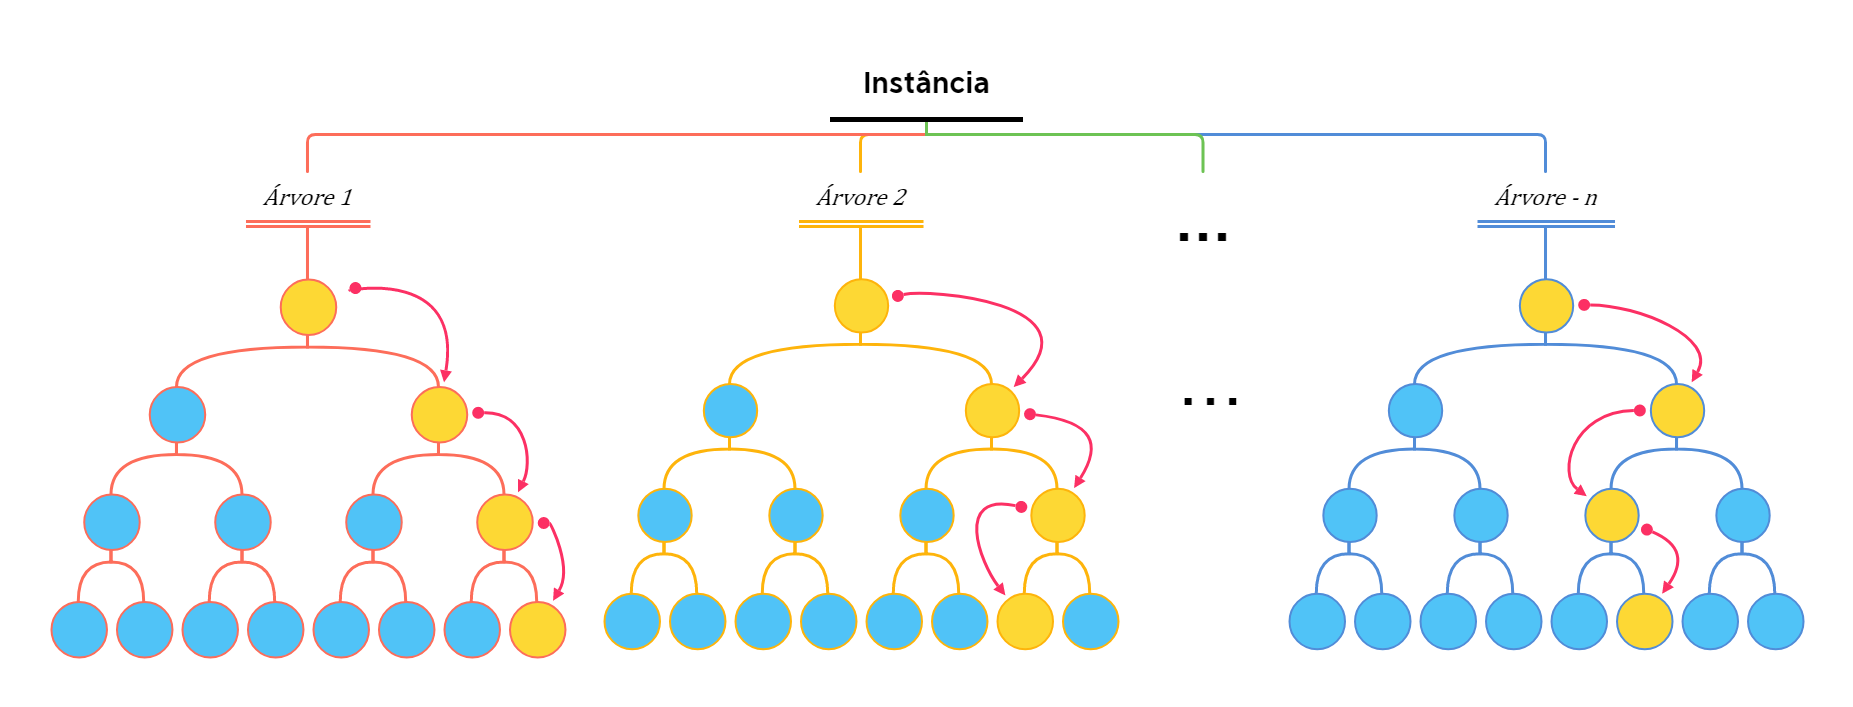
\includegraphics[width=0.9\linewidth]{Modelos/Figuras/RF}
	
	Fonte: Elaboração própria
\end{figure}


\subsubsection{Gradient Boosting (como XGBoost, LightGBM)}\label{subsubsec:lgbxgb}

O aumento de gradiente (do inglês\textit{gradient boosting}) é um método que combina vários modelos de árvore de decisão para realizar previsões. Cada uma dessas árvores de decisão é única, pois a diversidade é um elemento importante nesse processo. A diversidade é alcançada através de um processo chamado boosting, que é uma abordagem iterativa. O boosting adiciona modelos fracos ao conjunto de forma inteligente, dando mais peso aos pontos de dados que ainda não foram bem previstos. 

O processo de boosting melhora o conjunto ao focar nas partes dos dados que ainda não são compreendidas. A Figura \ref{fig:xgboost} apresenta uma visão esquemática desse processo. À medida que novos modelos fracos são adicionados, todos os modelos fracos intermediários são mantidos. O modelo final é uma combinação de todos esses modelos fracos, resultando em um ensemble que oferece uma melhor capacidade de previsão do que um único modelo.

O boosting é apenas um dos métodos de ensemble utilizados em conjunto com o bagging. O bagging também é um método que utiliza múltiplos modelos de árvore de decisão, porém, em vez de adicionar os modelos de forma iterativa, cada modelo é treinado independentemente em subconjuntos aleatórios dos dados de treinamento. Ambos os métodos, boosting e bagging, têm como objetivo melhorar o desempenho do modelo combinando as previsões de múltiplos modelos individuais.


\begin{figure}[H]
	\centering
	\caption{Impulsionando gradiente com XGBoost e LightGBM}
	\label{fig:xgboos}
	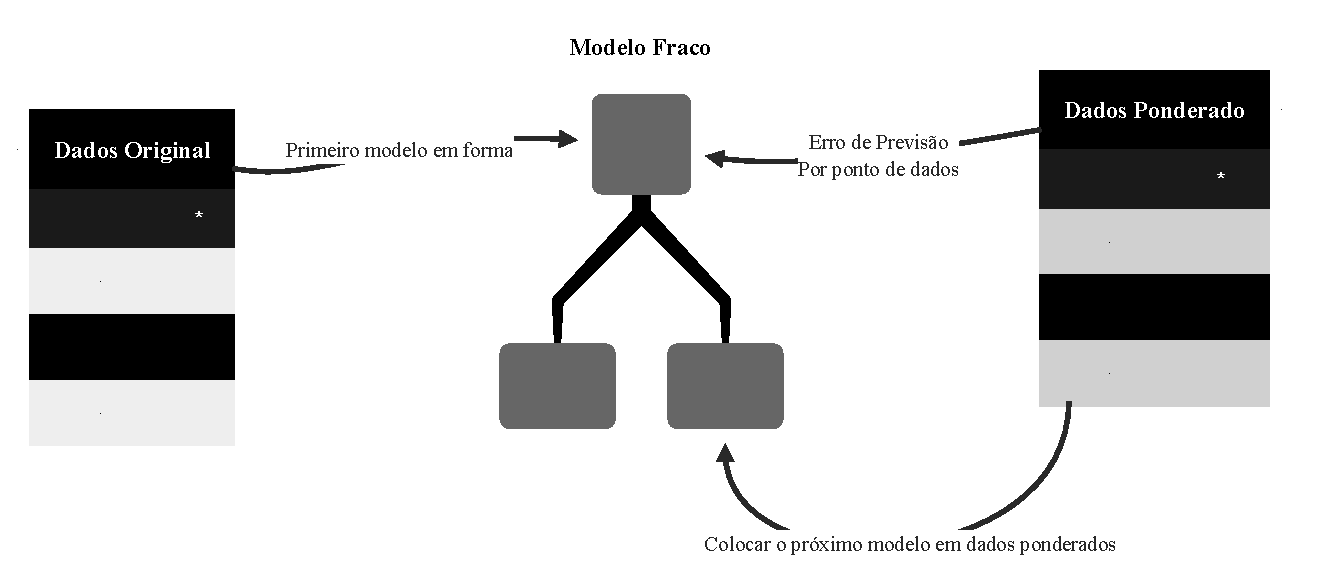
\includegraphics[width=0.9\linewidth]{Modelos/Figuras/xgboos}
	
	Fonte: Adaptação de \citeonline{korstanje2021}
\end{figure}



\subsubsection{O Gradiente em Gradiente de Boosting (Refor\c co)} \label{subsubsec:boosting}

O processo iterativo utilizado no aumento de gradiente, como descrito por \citeonline{korstanje2021}, recebe esse nome por um motivo. O termo ``gradiente'' refere-se a um campo vetorial de derivadas parciais que apontam na direção da inclinação mais acentuada. De forma simplificada, podemos pensar nos gradientes como as inclinações das estradas: quanto maior a inclinação, mais íngreme a colina. Para calcular os gradientes, são realizadas derivadas ou derivadas parciais de uma função.

No aumento de gradiente, ao adicionar árvores adicionais ao modelo, o objetivo é incorporar uma árvore que explique melhor a variação que ainda não foi explicada pelas árvores anteriores. Dessa forma, a nova árvore tem como objetivo ajustar-se aos erros ou resíduos deixados pelas árvores anteriores.

\begin{equation}
	y-\hat{y} \label{eq:xb}
\end{equation}

A equação \eqref{eq:xb} pode ser reescrita como a derivada parcial negativa da função de perda em relação às previsões $\hat{y}$:

\begin{equation}
	y-\hat{y} = -\frac{\partial L}{\partial \hat{y}} \label{eq:xb2}
\end{equation}

Isso é definido como o objetivo da nova árvore a ser adicionada no modelo de aumento de gradiente, garantindo que ela explique a máxima quantidade de variação adicional no modelo geral. Essa é a razão pela qual o modelo é chamado de "aumento de gradiente" (``\textit{gradient boosting}'', em inglês). O processo utiliza o gradiente da função de perda para guiar a adição de novas árvores, buscando minimizar o erro e melhorar a capacidade do modelo em explicar a variação nos dados.

\subsubsection{Algoritmos de boosting de gradiente}

Existem muitos algoritmos que executam versões ligeiramente diferentes de aumento de gradiente. Quando o método de aumento de gradiente foi inventado, o algoritmo não tinha um desempenho tão bom, mas isso mudou com o advento do algoritmo AdaBoost: o primeiro algoritmo capaz de se adaptar a modelos fracos.

O algoritmo de aumento de gradiente é uma das ferramentas de aprendizado de máquina com melhor desempenho no mercado. Após o AdaBoost, uma longa lista de algoritmos de aumento levemente diferentes foi adicionada à literatura, incluindo XGBoost, LightGBM, LPBoost, BrownBoost, MadaBoost, LogitBoost e TotalBoost. Ainda há muitas contribuições para melhorar a teoria do aumento de gradiente. Nesta subseção, dois algoritmos são apresentados: XGBoost e LightGBM.

O \textbf{XGBoost} é um dos algoritmos de aprendizado de máquina mais utilizados. É uma forma rápida de obter bom desempenho. Devido à sua facilidade de uso e alto desempenho, é frequentemente o primeiro algoritmo escolhido por muitos profissionais de aprendizado de máquina.

O \textbf{LightGBM} é outro algoritmo de aumento de gradiente que é importante conhecer. Atualmente, é um pouco menos difundido que o XGBoost, mas está ganhando popularidade rapidamente. A vantagem esperada do LightGBM em relação ao XGBoost é um ganho de velocidade e uma utilização mais eficiente de memória.

Nesta subseção, você encontrará as implementações de ambos os algoritmos de aumento de gradiente.

\subsubsection{A diferen\c ca entre XGBoost e LightGBM}

Se alguém planeja utilizar os dois algoritmos de aumento de gradiente, é importante que essa pessoa compreenda suas diferenças, o que também proporciona uma visão das várias divergências que existem entre os modelos disponíveis no mercado.

Uma diferença fundamental reside na maneira como esses algoritmos identificam as melhores divisões entre os nós das árvores de decisão individuais. É crucial lembrar que uma divisão em uma árvore de decisão ocorre quando a árvore precisa encontrar a separação que mais melhora o desempenho do modelo.

A abordagem intuitiva e simples para encontrar a melhor divisão é iterar por todas as possibilidades e selecionar a melhor. No entanto, essa abordagem é computacionalmente custosa, e algoritmos mais recentes apresentam alternativas mais eficientes.

Uma alternativa proposta pelo XGBoost é a segmentação baseada em histograma. Nesse caso, em vez de iterar por todas as partições possíveis, o modelo constrói um histograma para cada variável e utiliza-os para encontrar a melhor divisão geral entre as variáveis.

O LightGBM, desenvolvido pela Microsoft, adota uma abordagem mais eficiente para a definição das divisões. Essa abordagem é conhecida como amostragem unilateral baseada em gradiente (GOSS). O GOSS calcula o gradiente para cada ponto de dados e utiliza-o para filtrar os pontos de dados com gradientes baixos. Afinal, os pontos de dados com gradientes baixos já são bem compreendidos, enquanto aqueles com gradientes altos precisam ser melhor aprendidos.

O LightGBM também utiliza uma abordagem chamada Exclusive Feature Bundling (EFB), que acelera a seleção de muitas variáveis correlacionadas. Outra diferença é que o modelo LightGBM é adequado para o crescimento de folhas (leaf-wise growth), enquanto o XGBoost cultiva as árvores em níveis (level-wise growth). Essa diferença pode ser visualizada na Figura \ref{fig:xgboost}.

Essa diferença teoricamente favorece o LightGBM em termos de precisão, mas também apresenta um maior risco de overfitting (sobreajuste) quando há poucos dados disponíveis. Portanto, é importante que a pessoa considere essas distinções ao escolher entre os dois algoritmos de aumento de gradiente.

\begin{figure}[H]
	\centering
	\caption{Crescimento em folha versus crescimento em nível}
	\label{fig:xgboost}
	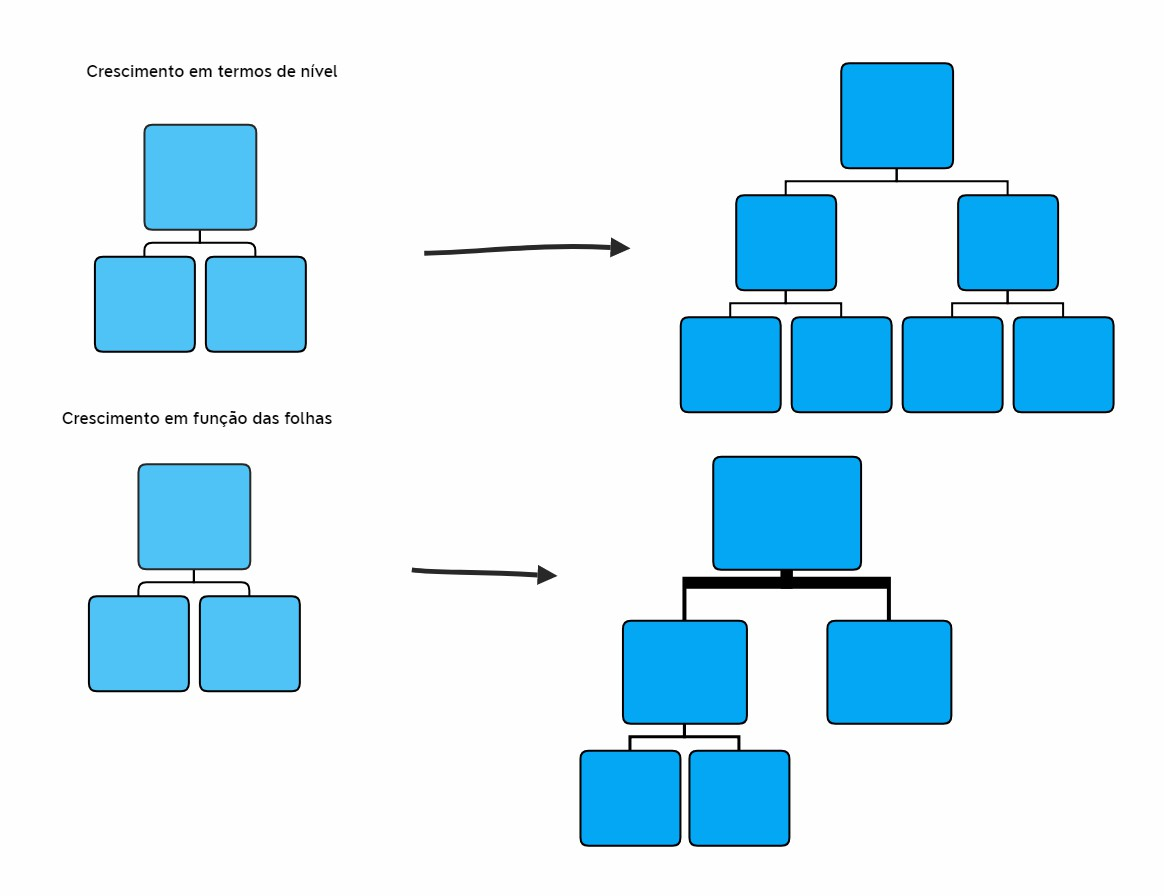
\includegraphics[width=0.9\linewidth]{Modelos/Figuras/xgboost}
	
	Fonte: Adaptação de \citeonline{korstanje2021}
\end{figure}


Na Figura \ref{fig:xgboost}, é possível visualizar como cada modelo é ajustado durante o processo de crescimento de árvore em folhas e em níveis. Essa representação gráfica oferece uma compreensão visual das diferenças entre os dois métodos.

No crescimento de árvore em folhas, como no LightGBM, novas folhas são adicionadas à árvore de forma iterativa, visando maximizar a redução do erro de treinamento. Isso significa que as árvores são expandidas adicionando folhas, uma a uma, até que o critério de parada seja alcançado.

Por outro lado, no crescimento em níveis, como no XGBoost, as árvores são expandidas em profundidade de forma simultânea em todos os níveis. Ou seja, em cada nível, todas as folhas são expandidas ao mesmo tempo, resultando em um crescimento mais uniforme da árvore.

Essa distinção no modo de crescimento das árvores pode afetar o comportamento e o desempenho do modelo. Portanto, compreender essa diferença é importante ao escolher entre esses algoritmos de aumento de gradiente.

\begin{figure}[H]
	\centering
	\caption{XGBoost e LigthGBM regressão}\label{fig:1-xgb-regressao}
	\includegraphics[width=0.9\linewidth]{Modelos/Figuras/0-xgb-regressão}
	
\end{figure}

\begin{figure}[H]
	\centering
	\includegraphics[width=0.9\linewidth]{Modelos/Figuras/0-lgbm-regressão}	
	
	
	Fonte: Elaboração própria a partir de dados da SANEPAR (2018 a 2020)
	
\end{figure}

Na Figura \ref{fig:1-xgb-regressao} é um modelo baseado nos dados coletados da SANEPAR.



\subsection{M\'etricas de Avalia\c c\~ao de Modelos}\label{subsec:metrica}

A métrica de Erro Quadrático Médio (MSE) é amplamente utilizada no campo do aprendizado de máquina para avaliar a qualidade dos modelos de previsão. O MSE é calculado pela média da soma dos quadrados das diferenças entre os valores reais e os valores previstos,

\begin{eqnarray}
	MSE &=& \frac{1}{n} \sum_{i=1}^{n} (y_i - \hat{y}_i)^2 \label{eq:mse}
\end{eqnarray}

\noindent onde, $n$ representa o número de amostras, $y_i$ é o valor real correspondente à amostra $i$ e $\hat{y}_i$ é o valor previsto para a mesma amostra. O MSE é calculado como a média das diferenças ao quadrado entre os valores reais e os valores previstos.

A utilização do MSE fornece uma medida quantitativa da precisão do modelo, pois penaliza de forma mais significativa os erros maiores. Ao elevar as diferenças ao quadrado, a métrica enfatiza a importância de minimizar as discrepâncias entre os valores reais e os valores previstos. Dessa forma, quanto menor o valor do MSE, melhor é o desempenho do modelo em termos de previsão.

Portanto, o MSE é uma métrica fundamental para avaliar a qualidade dos modelos de previsão e é amplamente utilizada para comparar diferentes algoritmos e abordagens de aprendizado de máquina.

\subsubsection{Erro Quadr\'atico M\'edio Raiz (RMSE)}

O RMSE é uma métrica amplamente empregada na avaliação de modelos de previsão em séries temporais. Ele é calculado tomando a raiz quadrada do MSE, conforme segue,

\begin{eqnarray}
	RMSE &=& \sqrt{\dfrac{1}{n} \sum_{i=1}^{n} (y_i - \hat{y}_i)^2} \label{eq:rmse}
\end{eqnarray}

\noindent onde \eqref{eq:rmse}, $n$ representa o número de amostras, $y_i$ é o valor real correspondente à amostra $i$, e $\hat{y}_i$ é o valor previsto para a mesma amostra. O RMSE fornece uma medida da dispersão média entre os valores reais e os valores previstos pelo modelo.

Uma das vantagens de utilizar o RMSE é que, ao computar a raiz quadrada, o erro passa a ter a mesma escala da variável de interesse. Isso permite uma interpretação mais fácil dos resultados, sendo que um valor baixo de RMSE indica um bom desempenho do modelo, já que o erro se aproxima de zero.

O RMSE possui algumas características positivas. Ele penaliza de forma significativa os valores discrepantes, caso seja necessário para o modelo. Além disso, o erro resultante está nas mesmas unidades da série temporal, facilitando a interpretação. O RMSE pode ser considerado uma combinação das melhores características do MSE e do Erro Absoluto Médio (MAE).

No entanto, o RMSE também apresenta algumas desvantagens. Ele tem uma interpretabilidade reduzida, uma vez que os erros ainda são elevados ao quadrado. Além disso, o RMSE é dependente da escala dos dados, o que impede sua comparação direta com modelos de séries temporais que utilizam unidades diferentes.

Apesar das limitações, o RMSE é uma métrica amplamente utilizada para avaliar modelos de previsão em séries temporais. Ele fornece uma medida da dispersão média entre os valores reais e previstos, auxiliando na compreensão do desempenho do modelo e na comparação com outras abordagens.

\subsubsection{Raiz do Erro M\'edio Quadr\'atico Relativo (RRMSE)}\label{subsub:rrmse}

\noindent\textbf{Vantagens do RRMSE :}


Interpretação intuitiva: O RRMSE é expresso como uma porcentagem, o que facilita a compreensão da precisão relativa do modelo. Quanto menor o valor do RRMSE, mais próximas estão as previsões dos valores reais.
	
Considera a escala dos dados: O RRMSE leva em consideração a magnitude dos erros em relação aos valores de referência. Isso é especialmente útil quando os dados têm uma grande variação e escala, pois evita que erros de grande magnitude dominem a avaliação.
	
Comparação entre modelos e algoritmos: O RRMSE pode ser usado para comparar a precisão de diferentes modelos ou algoritmos em um problema de regressão. Ao calcular o RRMSE para cada modelo, é possível identificar aquele que apresenta melhor desempenho em relação aos valores reais.
	
Sensibilidade relativa a diferentes magnitudes de erro: O RRMSE captura erros relativos em diferentes magnitudes. Isso significa que ele é capaz de identificar discrepâncias proporcionais, independentemente do valor absoluto dos erros.


\noindent\textbf{Desvantagens do RRMSE:}


Sensibilidade a \textit{outliers}: O RRMSE pode ser influenciado por valores discrepantes nos dados. Se houver valores extremos que não representem a tendência geral, o RRMSE pode ser distorcido, pois considera a média dos valores reais na fórmula de cálculo.
	
Necessidade de uma linha de base adequada: O RRMSE requer uma linha de base apropriada para comparação. Isso significa que é necessário ter um valor de referência confiável ou um modelo de referência para calcular o RRMSE e interpretar os resultados corretamente.
	
Foco exclusivo na precisão relativa: O RRMSE se concentra exclusivamente na precisão relativa e não leva em consideração outras métricas de desempenho, como tempo de execução, complexidade do modelo ou outros aspectos específicos do problema em questão. Portanto, é importante complementar o uso do RRMSE com outras métricas relevantes,





\begin{eqnarray}
	\text{RRMSE} &=& \left(\frac{\text{RMSE}}{\text{Média dos Valores Reais}}\right) \times 100 \label{eq:rrmse}
\end{eqnarray}


\noindent onde RMSE representa o Erro Médio Quadrático e ``Média dos Valores Reais'' denota a média aritmética dos valores reais no conjunto de dados.

É essencial que sejam consideradas essas vantagens e desvantagens ao utilizar o RRMSE como métrica de avaliação. Além disso, é recomendado o uso de várias métricas em conjunto para obter uma visão mais completa do desempenho do modelo de regressão.



\subsubsection{Erro Absoluto M\'edio (MAE)}

O Erro Absoluto Médio (MAE) é amplamente utilizado como uma métrica para avaliar o desempenho de modelos de previsão. Em vez de calcular a média das diferenças entre os valores reais e previstos, o MAE calcula a média dos valores absolutos dessas diferenças, garantindo que os erros positivos e negativos não se anulem.

O MAE mede o desvio médio das previsões em relação aos valores reais e é uma métrica intuitiva e fácil de interpretar, representando a magnitude média dos erros em relação à escala dos dados. Por exemplo, um MAE de 2 significa que, em média, as previsões têm um desvio absoluto de 2 unidades em relação aos valores reais.

Uma das vantagens do MAE é a sua insensibilidade a valores extremos, pois trata os erros de forma absoluta. No entanto, como o MAE não considera a magnitude dos erros individuais, pode não refletir adequadamente a gravidade de desvios significativos em relação aos valores reais.

Para superar essa limitação, uma alternativa é o Erro Médio Absoluto Percentual (MAPE). O MAPE expressa o MAE como uma porcentagem em relação aos valores reais, proporcionando uma medida relativa de erro. Essa métrica é especialmente útil quando se deseja avaliar o desempenho de um modelo em relação à magnitude dos dados.

Em resumo, o MAE é uma métrica simples e fácil de interpretar, que mede o desvio médio das previsões em relação aos valores reais. O MAPE, por sua vez, fornece uma medida relativa de erro, expressa como uma porcentagem dos valores reais. A escolha entre essas métricas depende do contexto do problema e dos requisitos específicos de avaliação.

O cálculo do MAE é realizado utilizando o valor absoluto da diferença entre o valor real e o valor previsto, e em seguida, divide-se pela quantidade $n$ de amostras. Isso resulta no erro médio absoluto. A equação do MAE é dada por:

\begin{eqnarray}
	M A E &=& \dfrac{1}{n} \sum\left|y_i-\hat{y}_i\right|\label{eq:mae}
\end{eqnarray}

Sua interpretação é similar ao RMSE, em que o erro é expresso na mesma escala ou ordem de grandeza da variável estudada.

\subsubsection{Erro Percentual Absoluto M\'edio (MAPE)}

O Erro Percentual Absoluto Médio (MAPE) é uma métrica que expressa o erro de previsão como uma porcentagem relativa ao valor observado. Ele é calculado somando as diferenças entre o valor real e o valor previsto (representando o erro), dividido pelo valor observado.
O MAPE é calculado usando a seguinte fórmula:

\begin{eqnarray}
	MAPE &=& \dfrac{1}{n} \sum\left|\frac{y_i - \hat{y}_i}{y_i}\right|\label{eq:mape}
\end{eqnarray}

No entanto, surge um problema quando o valor observado $y_i$ é igual a zero, pois é matematicamente impossível dividir por zero. O MAPE é uma medida de erro em que valores menores indicam um melhor desempenho de previsão.
Uma alternativa ao MAPE é calcular $1 - \text{MAPE}$, que representa a porcentagem de acerto.
O Erro Percentual Absoluto Médio é comumente usado como uma métrica de referência para avaliar o desempenho de modelos de previsão.

\noindent\textbf{Vantagens do MAPE:}


Fácil de interpretar.
Independente de escala, permitindo comparações entre diferentes séries temporais


\noindent\textbf{Desvantagens do MAPE:}

Erro infinito se o valor real estiver próximo ou igual a zero.
Previsões mais baixas estão propensas a ter um erro de 100\%, enquanto previsões mais altas podem ter um erro infinito, o que resulta em um viés de subprevisão.
Essa métrica são amplamente utilizadas na avaliação de modelos de previsão em diferentes áreas e ajudam a quantificar a qualidade das previsões realizadas pelos modelos.

\subsubsection{Erro Percentual Absoluto M\'edio Sim\'etrico (sMAPE)}


O sMAPE (do inglês \textit{Symmetric Mean Absolute Percentage Error}), ou Erro Médio Percentual Absoluto Simétrico, é outra métrica comumente utilizada para avaliar a precisão de modelos de previsão. Aqui estão as vantagens e desvantagens do sMAPE:

\noindent\textbf{Vantagens do sMAPE:}


Interpretação intuitiva: O sMAPE é expresso como uma porcentagem, facilitando a compreensão da precisão relativa do modelo. Valores menores indicam uma melhor precisão.	
Simetria: Ao contrário do MAPE (do inglês \textit{Mean Absolute Percentage Error}), o sMAPE é simétrico em relação aos valores previstos e reais. Isso significa que ele considera igualmente as discrepâncias de subestimação e superestimação.	
Robustez contra valores nulos: O sMAPE é adequado para lidar com valores nulos nos dados, pois a divisão por zero é evitada no cálculo da métrica.


\noindent\textbf{Desvantagens do sMAPE:}


Sensibilidade a valores extremos: O sMAPE é sensível a valores extremos nos dados. Se houver valores discrepantes que não representem a tendência geral, eles podem influenciar significativamente a métrica.	
Assimetria em torno de zero: Embora o sMAPE seja simétrico em relação aos valores previstos e reais, ele não é simétrico em torno de zero. Isso pode causar interpretações inconsistentes, especialmente quando os valores reais são próximos de zero.



\begin{eqnarray}
	sMAPE &=& \dfrac{1}{n} \sum_{i=1}^{n} \dfrac{2|y_i - \hat{y}_i|}{(|y_i| + |\hat{y}_i|)} \times 100\label{eq:smape}
\end{eqnarray}


\noindent onde $y_i$ representa o valor real, $\hat{y}_i$ representa o valor previsto e $n$ é o número total de amostras.
Ao utilizar o sMAPE como métrica de avaliação, é importante considerar esses prós e contras. Além disso, recomenda-se o uso de várias métricas em conjunto para obter uma visão abrangente do desempenho do modelo de previsão.






\subsection{Trabalhos Relacionados}\label{subsec:estudo-de-caso-base}


A previsão da demanda de água é uma preocupação fundamental para muitas organizações e autoridades responsáveis pelo abastecimento de água. A análise de séries temporais é uma abordagem comumente usada para prever padrões futuros com base em dados históricos. Neste estudo de caso, será explorado como a análise de séries temporais pode ser aplicada para prever a demanda de água ao longo do tempo.



Na subseção \ref{subsubsec:obespec} estão as perguntas de pesquisa que serão abordadas no estudo de caso, da pergunta \ref{q1} à \ref{q5}, com as ramificações da \ref{q5}.
Na subseção \ref{subsec:descricao}, são apresentadas as variáveis contidas no conjunto de dados coletado no período de $2018$ a $2020$, durante uma grave falta de água que afetou a cidade. Devido a essa situação, foi implementado um rodízio de abastecimento de água para os residentes. Os dados foram coletados em intervalos de uma hora, levando em consideração cada variável, com ênfase na variável-alvo, denominada LT01, que representa o nível do reservatório.

O conjunto de dados possui um total de $26.306$ linhas e $9$ colunas. Durante a coleta dos dados, verificou-se que eles apresentam padrões sazonais, indicando variações recorrentes ao longo do tempo. Além disso, constatou-se que o consumo diário foi significativamente afetado no ano de 2020, diferindo dos anos anteriores, nos quais as mudanças não foram tão significativas.

Ao longo do trabalho realizado, pôde-se observar na subseção \ref{subsec:detec} que foi realizada uma análise gráfica do problema antes da aplicação de qualquer método. A detecção de anomalias mostrou-se desafiadora, porém não impossível de ser realizada. Essa detecção permitiu a análise da presença de sazonalidade nos dados. A decomposição STL foi utilizada para essa finalidade, conforme descrito na etapa \ref{etp:3} e detalhado na subseção \ref{subsubsec:stl}, onde são apresentadas as decomposições realizadas.

É fundamental lembrar que, durante a análise exploratória, os dados sofreram algumas alterações. Por exemplo, a média diária foi calculada em vez de ser considerada a nível horário, resultando em uma redução do conjunto de dados de 26.306 linhas para 1.096 linhas. A decomposição STL foi aplicada nos formatos aditivo e multiplicativo, e ambas as abordagens estão ilustradas nas Figuras \ref{fig:stl-aditiva} e \ref{fig:stl}, respectivamente.
Adicionalmente, na subseção \ref{subsubsec:stl}, foi realizada a verificação da estacionariedade da série. O teste de DF (do inglês \textit{Dickey-Fuller}) foi empregado para auxiliar na tomada de decisões, e os resultados demonstraram que a série em análise é estacionária, conforme evidenciado pelo teste DF.


Dentro da análise, foram incluídos uma variedade de modelos para melhor capturar a natureza dos dados e aprimorar as previsões. Esses modelos incluem:
RNN, que leva em conta as dependências sequenciais nos dados para prever valores futuros.
LSTM, um tipo de RNN que lida especialmente bem com sequências longas e dependências de longo prazo.
GRU, outra variante de RNN que equilibra o poder de modelagem e a eficiência computacional.
Transformer, um modelo amplamente utilizado para tarefas de processamento de linguagem natural e sequências, que também pode ser adaptado para previsões sequenciais.
Prophet, um modelo de previsão desenvolvido pelo Facebook que lida bem com dados sazonais e tendências.
\textit{Decision Tree Regressor}, um modelo baseado em árvore de decisão que segmenta os dados em subgrupos para fazer previsões.
Esses modelos são complementados com abordagens tradicionais como:

Modelos de séries temporais univariados, incluindo AR, MA, ARMA, ARIMA e SARIMA, que levam em consideração a sazonalidade dos dados.
Modelos de séries temporais multivariados, como ARX, ARIMAX e SARIMAX, que incorporam variáveis exógenas para melhorar as previsões.
Foram explorados modelos de aprendizado de máquina supervisionados:

LR (\textit{Regressão Linear}), que estabelece relações lineares entre variáveis para fazer previsões.
RFR (\textit{Random Forest Regressor}), um \textit{ensemble} de árvores de decisão que captura complexas relações nos dados.
LightGBM e XGBoost, modelos baseados em \textit{gradient boosting} que são reconhecidos por sua eficácia na previsão e tomada de decisões. O XGBoost é particularmente conhecido por seu desempenho superior em várias métricas de avaliação.



\noindent\textbf{Ajuste do modelo}


Ao ajustar o modelo para a base de dados, foi feita uma alteração na ordem do modelo sugerido pelo \textbf{pmdarima}. A escolha foi trocar o modelo SARIMAX(1,1,1)(2,1,0,12) para SARIMAX(7,1,7)(2,1,0,12). Essa decisão foi tomada com base na observação de um ajuste mais preciso aos dados, evidenciado pela redução nos resíduos e uma melhor captura das características da série temporal. Além disso, considerando o conhecimento do problema e as características específicas dos dados, foi identificado que padrões mais complexos requeriam ordens mais altas para serem adequadamente capturados. Dessa forma, foi realizado um processo iterativo de experimentação e avaliação para determinar o modelo SARIMAX(7,1,7)(2,1,0,12) como o mais adequado para a base de dados em questão. É importante ressaltar que o desempenho do novo modelo será avaliado por meio de diagnósticos adicionais e análise dos resultados obtidos.

Os modelos RNN, LSTM e GRU foram ajustados minuciosamente por meio da técnica de otimização de hiperparâmetros do Optuna, permitindo uma exploração adaptativa e eficiente do espaço de configurações. Essa abordagem exclusiva do Optuna resultou em modelos sequenciais com aprimoramento notável na capacidade preditiva. Parâmetros vitais, como taxa de aprendizado, tamanho da camada oculta e número de unidades, foram otimizados de forma eficaz através do Optuna \cite{DBLP}.

O RFR apresentou melhorias notáveis após o ajuste com o Optuna. A otimização realizada pelo Optuna permitiu identificar uma combinação de hiperparâmetros ideal para o RFR, resultando em um significativo aprimoramento no desempenho preditivo desse modelo.
Considerando que o modelo LR não demonstrou melhorias significativas, uma decisão foi tomada para substituí-lo pelo modelo \textit{Decision Tree Regressor}. Este último foi ajustado empregando o Optuna, buscando encontrar a configuração de hiperparâmetros ideal para o modelo de árvore de decisão. Essa decisão foi respaldada pelo fato de que o Optuna havia demonstrado ser uma ferramenta eficaz para otimização de hiperparâmetros, como evidenciado pelas melhorias observadas no RFR e em outros modelos \cite{DBLP}.

Dessa forma, os modelos RNN, LSTM, GRU, XGBRegressor, LGBMRegressor e o Decision Tree Regressor foram todos otimizados com sucesso utilizando o Optuna, resultando em previsões mais robustas e confiáveis. No entanto, os modelos Transformer e Prophet mantiveram suas configurações originais devido à ausência de melhorias substanciais após tentativas de otimização com o Optuna.

O \textbf{Optuna} oferece uma abordagem de otimização de hiperparâmetros mais avançada e eficaz em comparação com outras técnicas amplamente utilizadas, como o GridSearchCV, BayesSearchCV e RandomizedSearchCV. Enquanto essas abordagens tradicionais têm suas vantagens, o Optuna leva a otimização de hiperparâmetros a um nível superior.
Existem geralmente dois tipos de métodos de amostragem: a amostragem relacional, que explora as correlações entre os parâmetros, e a amostragem independente, que recolhe amostras de cada parâmetro de forma independente. A amostragem independente não é necessariamente uma opção ingênua, porque alguns algoritmos de amostragem como o TPE A eficácia em termos de custos da amostragem relacional e independente depende do ambiente e da tarefa. O Optuna apresenta ambos, e pode lidar com vários métodos de amostragem independente independentes, incluindo TPE, bem como métodos de amostragem relacional como o CMA-ES. No entanto, há que ter algumas palavras de precaução para a implementação da amostragem relacional num definido por execução \cite{DBLP}.

\noindent\textbf{Avalia\c c\~ao do modelo}


A avaliação da precisão dos modelos de previsão é uma etapa fundamental no processo de modelagem. Diversas métricas podem ser utilizadas para esse propósito, como o sMAPE, o MAE e o RRMSE. Essas métricas têm sido amplamente adotadas na literatura de previsão e são consideradas indicadores confiáveis para mensurar a qualidade das previsões.

O MAPE é uma métrica bastante utilizada na avaliação de modelos de previsão, especialmente quando há variações significativas nos dados ou quando se deseja comparar a precisão de diferentes modelos. O MAPE calcula o erro médio percentual entre as previsões e os valores reais, fornecendo uma medida relativa da precisão do modelo \cite{zhang2016}.
O uso do erro médio absoluto (MAE) apresenta vantagens na avaliação do desempenho médio de um modelo, em comparação com o erro quadrático médio (RMSE) \cite{willmott2005advantages}.
Destacam a importância do RMSE na avaliação de modelos e argumentam contra a exclusão dessa métrica na literatura \cite{jones2017}.


O RRMSE é uma métrica de avaliação altamente eficaz para medir a precisão relativa de modelos de regressão. Eles destacam que sua normalização em relação à média dos valores reais permite uma interpretação intuitiva e facilita a comparação entre diferentes modelos. Segundo os autores, o RRMSE é amplamente utilizado na literatura devido à sua capacidade de fornecer uma medida robusta e padronizada da precisão dos modelos de regressão \cite{lopes2020evaluation}. O MAPE é amplamente utilizado na avaliação de modelos de previsão, especialmente quando há variações significativas nos dados ou quando se deseja comparar a precisão de diferentes modelos \cite{peng2017effective}.

O sMAPE é uma métrica amplamente utilizada para avaliar a precisão de modelos de previsão. Eles afirmam que o sMAPE possui algumas vantagens, como a consideração da simetria dos erros percentuais e a interpretação intuitiva como uma medida de precisão relativa \cite{nguyen2020toxicological}.

O MAE e o RMSE são métricas amplamente adotadas na análise de previsões, pois fornecem uma medida direta do desvio absoluto e do desvio quadrático médio entre as previsões e os valores observados. O MAE é particularmente útil quando se busca uma medida de erro que não seja sensível a valores extremos, enquanto o RMSE penaliza de forma mais significativa os erros maiores, oferecendo uma visão mais abrangente da precisão do modelo \cite{jones2017}.

O sMAPE é uma métrica de avaliação popular para comparar a precisão de diferentes modelos de previsão. Eles destacam que o sMAPE é particularmente útil quando os valores de demanda têm diferentes magnitudes, pois captura os erros relativos em uma escala percentual. Além disso, o sMAPE possui uma interpretação intuitiva e facilita a comparação entre modelos de previsão \cite{hyndman2006effect}.

\subsubsection{Estudo de Caso 1}

\noindent\textbf{Estudo de Caso 1: Adequação da Pressão e Vazão em uma Rede de Distribuição de Água}

\eqref{q1} Adequação da pressão atual para atender à demanda diária: Neste estudo de caso, o modelo SARIMAX (H) foi utilizado para avaliar a adequação da pressão atual em uma rede de distribuição de água, considerando a demanda diária \cite{2-s2.0-85099424908}. O objetivo foi prever a pressão na rede com base em dados históricos, permitindo que fosse realizada uma análise crítica da capacidade do sistema em atender às necessidades dos consumidores.

\eqref{q2} Volume mínimo de água no reservatório para evitar o acionamento das bombas: Para determinar o volume mínimo de água necessário no reservatório para evitar o acionamento das bombas durante o horário de pico, foi empregado um modelo Decision Tree Regressor (I) \cite{2-s2.0-85054695177}. Este modelo ajudou a identificar regras e padrões que guiam a tomada de decisão sobre o nível de armazenamento ideal.

\eqref{q3} Vazão ótima para atender à demanda diária: O estudo também buscou encontrar a vazão ótima para atender à demanda diária. Para isso, utilizou-se o modelo XGBRegressor (K) para otimizar a vazão na rede de distribuição, considerando as flutuações na demanda ao longo do dia \cite{2-s2.0-85130441623}.

\subsubsection{Estudo de Caso 2}

\noindent\textbf{Estudo de Caso 2: Impacto do Acionamento das Bombas durante o Horário de Pico em uma Rede de Distribuição de Água}

\eqref{q5} Impacto do acionamento das bombas durante o horário de pico: Neste segundo estudo de caso, analisou-se o impacto do acionamento das bombas durante o horário de pico em uma rede de distribuição de água.

\ref{q5}\eqref{q5:a} Nível ideal no reservatório e variação das vazões nos horários críticos: Utilizou-se o modelo ARIMA (E) \cite{2-s2.0-85069459067} para prever o nível ideal no reservatório e analisar as variações das vazões nos horários críticos, levando em consideração as diferentes estações do ano.

\ref{q5}\eqref{q5:b} Tendência, padrão e sazonalidade nos dados do Bairro Alto: Para identificar tendências, padrões e sazonalidades nos dados de três anos do Bairro Alto, empregou-se o modelo de decomposição STL, reconhecido por sua eficácia na modelagem de séries temporais com essas características.

\ref{q5}\eqref{q5:c} Identificação dos horários de maior demanda: A identificação dos horários de maior demanda entre as 18h e as 21h foi realizada com o uso da RNN (P) \cite{2-s2.0-85067419084}.

\ref{q5}\eqref{q5:d} Tendência, padrão e sazonalidade nos dados do Bairro Alto: Para identificar tendências, padrões e sazonalidades nos dados de três anos do Bairro Alto, empregou-se o modelo decomposição STL, reconhecido por sua eficácia na modelagem de séries temporais com essas características. Volume de armazenamento no reservatório para evitar o acionamento das bombas: Determinar a quantidade de água a ser armazenada previamente no reservatório para evitar o acionamento das bombas durante o horário de pico envolveu o modelo LGBMRegressor (L).

\ref{q5}\eqref{q5:e} Tendência, Padrão e Sazonalidade nos Dados do Bairro Alto: Para identificar tendências, padrões e sazonalidades nos dados de três anos do Bairro Alto, empregou-se o modelo STL, reconhecido por sua eficácia na modelagem de séries temporais com essas características. Detecção de anomalias na rede com base no histórico): Para detectar anomalias na rede com base no histórico de vazão e pressão, utilizou-se novamente o modelo ARX (B) \cite{2-s2.0-85051469381}.












